\chapter{Tracking of Charged Particles}
\label{c:charged.track}

\bmad can track both charged particles and X-rays. This chapter deals with charged particles and
X-rays are handled in chapter~\sref{c:xray.track}.

For tracking and transfer map calculations (here generically called ``tracking''), \bmad has various
methods that can be applied to a given element (Cf. Chapter~\sref{c:methods}). This chapter
discusses the \vn{bmad_standard} calculation that is the default for almost all element types and
the \vn{symp_lie_bmad} calculation that does symplectic integration.

Generally, it will be assumed that tracking is in the forward direction.

%-----------------------------------------------------------------
\section{Relative Versus Absolute Time Tracking}
\label{s:rf.time}

\index{relative time tracking}\index{absolute time tracking}
\index{lcavity}\index{rfcavity}\index{em_field}
Unlike other elements, the kick given a particle going through an \vn{lcavity}, \vn{rfcavity}, or
possibly an \vn{em_field} element depends upon the time that the particle enters the element
relative to some ``RF clock''. \bmad has two modes for calculating this time called ``\vn{relative
time tracking}'' and ``\vn{absolute time tracking}''. The switch to set the type of tracking for a
lattice is \vn{bmad_com[absolute_time_tracking]} (\sref{s:bmad.common}).\footnote
  {
An old, deprecated notation for this switch is \vn{parameter[absolute_time_tracking]}.
  }
The phase of the RF, $\phi_\text{rf}$, is determined by
\begin{equation}
  \phi_\text{rf} = \phi_\text{t} + \phi_\REF
\end{equation}
where $\phi_\text{t}$ is the part of the phase that depends upon the time $t$ and $\phi_\REF$
is a fixed phase offset (generally set in the lattice file) and independent of the particle
coordinates. See \Eqs{lcav.phi} and \eq{rfcav.phi}

The phase $\phi_\text{t}$ is 
\begin{equation}
  \phi_\text{t} = f_\text{rf} \ t_\text{eff}
\end{equation}
where $f_\text{rf}$ is the RF frequency, and $t_\text{eff}$ is the effective time. With \vn{relative
time tracking}, which \bmad uses by default, $t_\text{eff}$ is a function of the 
phase space coordinate $z$ (\sref{s:phase.space}) via
\begin{equation}
  t_\text{eff}(s) = t_0(s) - t_0(s_\text{ent}) - \frac{z(s)}{\beta \, c}
  \label{tttz}
\end{equation}
where $t_0$ is the reference time (see \Eq{zbctt}) and $s_\text{ent}$ is the $s$-position at the
upstream end of the element. $t_\text{eff}$ is defined such that a particle entering an element 
with $z = 0$ has $t_\text{eff} = 0$.

With \vn{absolute time tracking}, and \vn{bmad_com[absolute_time_ref_shift]} set to True (the
default), $t_\text{eff}$ is defined by
\begin{equation}
  t_\text{eff}(s) = t(s) - t_0(s_\text{ent})
\end{equation}
$t_0(s_\text{ent})$, by definition, equal to the time of the reference particle at the entrance end
of the element. With multipass \sref{c:multipass}, $t_0(s_\text{ent})$ is set by the time of the
reference particle at the entrance end of the element on the first pass. For absolute time tracking,
it is important to keep in mind that $t_0(s_\text{ent})$ is a property of the element independent of
how tracking is done. Thus, if a particle goes through a particular element multiple times, the
value of $t_\text{ent}$ will be the same for each transit. If \vn{bmad_com[absolute_time_ref_shift]}
set to False, $t_\text{eff}$ is simply
\begin{equation}
  t_\text{eff}(s) = t(s) 
\end{equation}

To understand the difference between relative and absolute time tracking, consider a particle
traveling on the reference orbit along side the reference particle in a circular ring with one RF
cavity. This particle always has $z = 0$ and thus, with \vn{relative time tracking}, $t_\text{eff}$
will always be zero (assuming \vn{bmad_com[absolute_time_ref_shift]} is set to True) at the entrance
to the cavity.  On the other hand, with \vn{absolute time tracking}, the particle, on the first
turn, will have $t_\text{eff}$ equal to zero. However, on subsequent turns (or subsequent passes if
using multipass), the time will increase by the revolution time $t_\text{C}$ on each turn. If the RF
frequency $f_\text{rf}$ is some multiple of the revolution harmonic, the RF phase with absolute vs
relative time tracking will be some multiple of $2 \, \pi$ and thus RF kick given the particle will
be the same in both cases. However, if the RF frequency is not some multiple of the revolution
harmonic, there will be a difference in the RF kicks (except for the kick on the first turn).

There are advantages and disadvantages to using either relative or absolute time tracking. Absolute
time tracking is more correct since RF cavities may have frequencies that are not commensurate with
the revolution time. The problem with absolute time tracking is that the transfer map through the
cavity is now a function of time and therefore is a function of $z$ {\em and} the turn number. This
complicates lattice analysis. For example, standard element transfer maps use phase space
coordinates so with absolute time tracking, one has a different map for each turn.

With relative time tracking the transfer map problem is swept under the rug. The penalty for using
relative time tracking is that results can be unphysical. For example, with relative time tracking,
the closed orbit is essentially independent of the RF frequency. In an actual machine, the closed orbit
will vary with RF frequency and, in fact, varying the RF frequency is one way of measuring
the dispersion. From a different angle this independence can be
viewed as a desirable feature since if one is only interested in, say, calculating the Twiss
parameters, it can be an annoyance to have to worry that the ring one has constructed have a length
that is exactly commensurate with the RF frequency. And it is potentially confusing to see non-zero
closed orbits when one is not expecting it due to a mismatch between the ring circumference and the
RF frequency or due to RF cavities not being spaced a multiple of the RF wavelength apart.

The above discussion is limited to the cavity fundamental mode. Long-range wakefields, on the
other hand, cannot be synchronized to the $z$ coordinate since, in general, their frequencies are
not commensurate with the fundamental mode frequency. For simulating the long-range wakes, the kick
is thus, by necessity, tied to the absolute time.

Do not confuse absolute time tracking with the \vn{time_runge_kutta} tracking method
(\sref{s:tkm}). The \vn{time_runge_kutta} method uses time as the independent variable instead of
$z$. Absolute time tracking just means that the RF phase is dependent upon the time instead of
$z$. It is perfectly possible to use absolute time tracking with code that uses $z$ as the
independent variable.

One important point to always keep in mind is that any PTC based tracking (\sref{s:ptc.intro}) will
always use relative time tracking independent of the setting of \vn{bmad_com[absolute_time_tracking]}.

%-------------------------------------------------------------------------
%-------------------------------------------------------------------------
\section{Element Coordinate System}
\label{s:ele.coords}

\index{element coordinates}
The general procedure for tracking through an element makes use of \vn{element reference}
coordinates (also called just \vn{element} coordinates). Without any offsets, pitches or tilt
(\sref{s:offset}), henceforth called ``misalignments'', the \vn{element} coordinates are the same as
the \vn{laboratory reference} coordinates (or simply \vn{laboratory} coordinates)
(\sref{s:ref}). The \vn{element} coordinates stay fixed relative to the element. Therefore, if the
element is misaligned, the \vn{element coordinates} will follow as the element shifts in the
laboratory frame as shown in \fig{f:ele.coord}.

Tracking a particle through an element is a three step process:
\begin{enumerate}
\item
At the entrance end of the element, transform from the \vn{laboratory} coordinates to the entrance
\vn{element} coordinates.
\item
Track through the element ignoring any misalignments. 
\item
At the exit end of the element, transform from the exit \vn{element} reference frame to the
\vn{laboratory} reference frame.
\end{enumerate}

The transformation between \vn{laboratory} and \vn{element} reference frames is given in
\sref{s:straight.mis} and \sref{s:bend.mis}.

%-------------------------------------------------------------------------

\begin{figure}[tb]
  \centering
  \includegraphics[width=5in]{coord-offset.pdf}
  \caption[Element Coordinate System.]
  {
\vn{Element} coordinates are coordinates attached to the physical element (solid green outline). The
\vn{laboratory} coordinates are fixed at the nominal position of the element (red dashed outline).
  }
  \label{f:ele.coord}.
\end{figure}

%-------------------------------------------------------------------------
\section{Hamiltonian}
\label{s:mag.hamiltonian}
The time dependent Hamiltonian $H_t$ in the curvilinear coordinate system shown
in \fig{f:local.coords} is (\cite{b:ruth})
\begin{equation}
  H_t = \wt\psi + \left[ \left( \frac{p_s - a_s}{1 + g\, x} \right)^2 + \wt m^2 + 
  (p_x - a_x)^2 + (p_y - a_y)^2 \right]^{1/2}
\end{equation}
where $(p_x, p_y, p_s/(1+gx))$ are the momentum normalized by $P_0$, $\rho$ being the local radius
of curvature of the reference particle, and $\wt m$, $\Bf a$ and $\wt\psi$ are the normalized mass,
vector, and scalar potentials:
\begin{equation}
  \wt m = \frac{m \, c^2}{c \, P_0} \qquad
  \left( a_x, a_y, \frac{a_s}{1+g \, x} \right) = \frac{q \, \Bf A}{P_0} \qquad 
  \wt\psi(x,y,z) = \frac{q \, \psi}{P_0 \, c}
  \label{mmccp}
\end{equation}
In terms of the normalized velocities $\beta_x$, $\beta_y$, the canonical momentum are
\begin{equation}
  p_x = \frac{m \, c^2}{P_0 \, c} \, \gamma \, \beta_x + a_x, \qquad 
  p_y = \frac{m \, c^2}{P_0 \, c} \, \gamma \, \beta_y + a_y
  \label{pmc2pc}
\end{equation}

The $s$-dependent Hamiltonian is obtained from $H_t$ by solving for
$-p_s$ and using a contact transformation to convert to \bmad
coordinates (\sref{s:phase.space}). For particles propagating in the
positive $s$ direction, the $s$-dependent Hamiltonian is, assuming
$\wt\psi$ is zero
\begin{equation}
  H \equiv H_s = -(1 + g \, x) \sqrt{(1 + p_z)^2 - (p_x - a_x)^2 - (p_y - a_y)^2} - 
  a_s + \frac{1}{\beta_0} \, \sqrt{(1+p_z)^2 + \wt m^2}
  \label{h1gx1}
\end{equation}
where $\beta_0$ is the reference velocity and the equality $(1 +
p_z)^2 = (E/c\, P_0)^2 - \wt m^2$ has been used. The last term on the
RHS of \Eq{h1gx1} accounts for the fact that the \bmad canonical $z$
(\Eq{zbctt}) has an ``extra'' term $\beta \, c \, t_0$ so that \bmad
canonical $z$ is with respect to the reference particle's $z$.

The equations of motion are
\begin{equation}
  \frac{dq_i}{ds} = \frac{\partial H}{\partial p_i} \qquad
  \frac{dp_i}{ds} = -\frac{\partial H}{\partial q_i}
  \label{rshp}
\end{equation}

\label{paraxial approximation} Without an electric field, $\psi$ is zero. Assuming a
non-curved coordinate system ($g = 0$), and using the paraxial approximation (which
expands the square root in the Hamiltonian assuming the transverse momenta are small)
(\sref{s:phase.space}), \Eq{h1gx1} becomes
\begin{equation}
  H = \frac{(p_x - a_x)^2}{2 (1 + p_z)} + \frac{(p_y - a_y)^2}{2 (1 + p_z)} - 
  (1 + p_z) - a_s +   \frac{1}{\beta_0} \, \sqrt{(1+p_z)^2 + \wt m^2}
  \label{hpapa}
\end{equation}

Once the transverse trajectory has been calculated, the longitudinal position
$z_2$ at the exit end of an element is obtained from symplectic
integration of \Eq{hpapa}
\begin{equation}
  z_2 = z_1 - \frac{1}{2 (1 + p_{z1})^2} \int \! ds \, 
  \left[ (p_x - a_x)^2 + (p_y - a_y)^2 \right] - \int \! ds \, g \, x
  \label{zz121p}
\end{equation}
where $z_1$ is the longitudinal position at the entrance end of the element.
Using the equations of motion \Eqs{rshp} this can also be rewritten as
\begin{equation}
  z_2 = z_1 - \frac{1}{2} \int \! ds \, 
  \left[ \left( \frac{dx}{ds} \right)^2 + \left( \frac{dy}{ds} \right)^2 \right] - 
  \int \! ds \, g \, x
  \label{zz12sx}
\end{equation}

For some elements, \vn{bmad_standard} uses a truncated Taylor map for
tracking.  For elements without electric fields where the particle
energy is a constant, the transfer map for a given coordinate $r_i$
may be expanded in a Taylor series
\begin{equation}
  r_{i,2} \rightarrow m_i + \sum_{j = 1}^4 m_{ij} \, r_{j,1} + 
  \sum_{j = 1}^4 \sum_{k = j}^4 m_{ijk} \, r_{j,1} \, r_{k,1} + \ldots
\end{equation}
where the map coefficients $m_{ij\cdots}$ are functions of $p_z$.  For
linear elements, the transfer map is linear for the transverse
coordinates and quadratic for $r_i = z$.

Assuming mid--plane symmetry of the magnetic field, so
that $a_x$ and $a_y$ can be set to zero\cite{b:madphysics}, The vector
potential up to second order is (cf.~\Eq{byx0b})
\begin{equation}
  a_s = -k_0 \left( x - \frac{g \, x^2}{2 (1 + g\, x)} \right) -
  \frac{1}{2} k_1 \left( x^2 - y^2 \right)
  \label{akxgx}
\end{equation}

For backwards propagation, where particle are traveling in the $-\Bf
s$ direction and where $p_s$ is negative, solving for $p_s$ involves
using a different part of the square root branch. There is also an
overall negative sign coming from switching from using $s$ as the
independent variable to $\wt s \equiv -s$ as the independent
variable. the Hamiltonian $H_{\wt s}$ is then
\begin{equation}
  H_{\wt s} = -(1 + g \, x) \sqrt{(1 + p_z)^2 - (p_x - a_x)^2 - (p_y - a_y)^2} + 
  a_s + \frac{1}{\beta_0} \, \sqrt{(1+p_z)^2 + \wt m^2}
\end{equation}

%---------------------------------------------------------------------------------
%---------------------------------------------------------------------------------
\section{Symplectic Integration}
\label{s:symp.track}
\index{symplectic integration}

Using \Eq{hpapa} the Hamiltonian is written in the form
\begin{equation}
  H = H_x + H_y + H_z
\end{equation}
where
\begin{equation}
  H_x = \frac{(p_x - a_x)^2}{2 (1 + \delta)}, \qquad
  H_y = \frac{(p_y - a_y)^2}{2 (1 + \delta)}, \qquad
  H_s = - a_s 
\end{equation}

For tracking, the element is broken up into a number of slices set by
the element's \vn{ds_step} attribute. For each slice, the tracking
uses a quadratic symplectic integrator $I$:
\begin{equation}
  I = T_{s/2} \; I_{x/2} \; I_{y/2} \; I_s \; I_{y/2} \; I_{x/2} \; T_{s/2}
\end{equation}
$T_{s/2}$ is just a translation of the $s$ variable:
\begin{equation}
  s \rightarrow s + \frac{ds}{2}
\end{equation}
And the other integrator components are
\begin{align}
  I_{x/2} &= \exp \left( : -\frac{ds}{2} H_x : \right) \CRNO
  I_{y/2} &= \exp \left( : -\frac{ds}{2} H_y : \right) \\
  I_{s}   &= \exp \left( : -ds \, H_s : \right) \nonumber
\end{align}
The evaluation of $I_{x/2}$ and $I_{y/2}$ is tricky since it involves both transverse
position and momentum variables. The trick is to split the integration into three parts.
For $I_{x/2}$ this is
\begin{align}
  I_{x/2} &= \exp \left( : -\frac{ds}{2} \frac{(p_x - A_x)^2}{2 (1 + \delta)} : \right) \CRNO
  &= \exp \left( : -\int A_x \, dx : \right) \,
     \exp \left( : -\frac{ds}{2} \frac{p_x^2}{2 (1 + \delta)} : \right) \,
     \exp \left( : \int A_x \, dx : \right)
  \label{ids2}
\end{align}
With an analogous expression for $I_{y/2}$.

\index{quadrupole}\index{sextupole}\index{wiggler}
For magnetic elements that do not have longitudinal fields
(quadrupoles, sextupoles, etc.), $a_x$ and $a_y$ can be taken to be
zero (cf.~\Eq{akxgx}).

\index{lcavity}\index{rfcavity}
For \vn{lcavity} and \vn{rfcavity} elements, the vector potential is computed from
\Eq{aiew}.

%---------------------------------------------------------------------------------
%---------------------------------------------------------------------------------
\section{BeamBeam Tracking}
\label{s:beambeam.std}
\index{beambeam}

A beam-beam element (\sref{s:beambeam}) simulates the effect on a tracked particle of an opposing
beam of particles moving in the opposite direction. The opposing beam, called the ``strong'' beam,
is assumed to be Gaussian in shape.

The strong beam is divided up into \vn{n_slice} equal charge (not equal thickness) slices.
Propagation through the strong beam involves a kick at the charge center of each slice with drifts
in between the kicks. The kicks are calculated using the standard Bassetti--Erskine complex error
function formula\cite{b:talman}.  Even though the strong beam can have a finite \vn{sig_z}, the
length of the element is always considered to be zero. This is achieved by adding drifts at either
end of any tracking so that the longitudinal starting point and ending point are identical. The
longitudinal $s$--position of the \vn{BeamBeam} element is at the center of the strong bunch. For
example, with \vn{n_slice} = 2 and with a solenoid field, the calculation would proceed as follows:
\begin{enumerate}[topsep=-0.2ex,itemsep=-0.0ex]
  \item 
Start with the particle longitudinally at the \vn{beambeam} element (which is considered to have
zero longitudinal length) in laboratory coordinates (\sref{s:coords.3}).
  %
  \item
Propagate backwards through the solenoid field so that the particle is in the plane of the first
beambeam slice. The fact that the plane of the slice may be, due to finite \vn{x_pitch} or
\vn{y_pitch} values, canted with respect to the laboratory $x$-$y$ plane is taken into account.
  %
  \item
Transform the particle coordinates to the \vn{beambeam} element body coordinates
(\sref{s:lab.body.transform}).
  %
  \item
Apply the beam--beam kick due to the first slice including a spin rotation.
  %
  \item
Transform back to laboratory coordinates.
  %
  \item
Propagate forwards so that the particle is in the plane of the second slice.
  %
  \item
Transform the particle coordinates to the \vn{beambeam} element body coordinates.
  %
  \item 
Apply the beam--beam kick due to the second slice.
  %
  \item 
Transform back to laboratory coordinates.
  %
  \item 
Propagate backwards through the solenoid field to end up with the particle longitudinally at the
\vn{beambeam} element.
  %
\end{enumerate}

There is an energy kick due to the motion of the strong beam. There are two parts to this $dp_z =
dp_{z,s} + dp_{z,h}$. One part, $dp_{z,s}$, is similar to the gravitational slingshot in orbital
mechanics. The slingshot energy kick is simply calculated using conservation of 4-momentum of the
tracked particle and the strong beam where the mass of the strong beam is assumed to be large
compared to the mass of the tracked particle.\footnote
  {
This assumption breaks down if a tracked particle is deflected due to a single scattering event with
a particle of the strong beam.  But particle-particle scattering is outside of the assumption of a
strong beam that is unaffected by the weak beam.
  }
After a little bit of algebra. The energy kick $dE_w$ to lowest order in the angle of the weak
particle with respect to the axis defined by the of motion of the strong beam is
\begin{equation}
  dE_w = \frac{c \, P_w}{2 \, (1/\beta_w + 1/\beta_s)} \, \left( \theta_{w2}^2 - \theta_{w1}^2 \right)
\end{equation}
where $P_w$ is the momentum of the weak particle, $\beta_w$ and $\beta_s$ are the weak and strong
beam velocities, and $\theta_{w1}$ and $\theta_{w2}$ are angles of the weak particle trajectory with
respect to the strong beam motion before and after the interaction. Converting to phase space
coordinates, the momentum kick $dp_z$ is
\begin{equation}
  dp_{z,s} = \frac{1}{2 \, \beta_w \, (1/\beta_w + 1/\beta_s) \, (1 + p_z)} 
    \left( dp_x \, (dp_x + 2p_{x1}) + dp_y \, (dp_y + 2p_{y1}) \right)
    \label{dpz12}
\end{equation}
where $dp_x$ and $dp_y$ are the transverse kicks and $p_{x1}$ and $p_{y1}$ are the initial phase
space momenta.

The other part of the energy kick, $dp_{z,h}$, happens when the strong beam's cross-section is changing due to
the hourglass effect. The hourglass longitudinal kick relative to the transverse kicks can derived using
Eq.~(5) of Sagan \cite{b:beamion}. In the relativistic limit the result is
\begin{equation}
  dp_{z,h} = \frac{\sigma_x}{2} \, \frac{d\sigma_x}{ds} \, \frac{dp_x}{dx} + 
             \frac{\sigma_y}{2} \, \frac{d\sigma_y}{ds} \, \frac{dp_y}{dy}
  \label{dpzsx}
\end{equation}
where $\sigma_x$ and $\sigma_y$ are the strong beam sizes, and the factor of two is due to the
relative velocity ($2c$) between the beams.

\newpage  % If newpage is removed, the footnote get put on the next page!!

%---------------------------------------------------------------------------------
%---------------------------------------------------------------------------------
\section{Bend: Exact Body Tracking with k1 = 0}
\label{s:bend.body.std}
\index{sbend}

\begin{figure}[h]
  \centering
  \includegraphics[width=5in]{bend-exact.pdf}
  \caption{Geometry for the exact bend calculation.}
  \label{f:bend.exact}
\end{figure}


Function definitions:
\begin{align}
  \sinc(x) &\equiv \frac{\sin(x)}{x} \\
  \cosc(x) &\equiv \frac{1 - \cos(x)}{x^2}
\end{align}
These functions cannot be directly evaluated at $x = 0$ and are defined at $x = 0$ using the $x
\rightarrow 0$ limit. The point to keep in mind here is that these functions are well behaved and
can be easily coded in software.

Referring to Figure~\ref{f:bend.exact}, at point 1 where the particle enters a sector bend, the angle
$\phi_1$ of the particle trajectory in the $(x,s)$ plane with respect to the $s$ axis is
\begin{equation}
  \sin(\phi_1) = \frac{p_{x1}}{\sqrt{(1+p_z)^2 - p_y^2}}
\end{equation}
where the subscript ``1'' for $p_z$ and $p_y$ is dropped since these quantities are invariant.

The $(u,v)$ coordinate system in the plane of the bend is defined with the $u$-axis along the exit
edge of the bend and the $v$-axis is perpendicular to the $u$-axis. The origin is at the design
center of the bend. In this coordinate system the point $(u_1, v_1)$ where the particle enters the
bend is given by
\begin{align}
  u_1 &= (\rho + x_1) \, \cos(\theta) \\
  v_1 &= (\rho + x_1) \, \sin(\theta)
\end{align}
where $\rho$ is the design radius of curvature, $x_1$ is the offset of the particle from the design
at the entrance point, and $\theta$ is the design bend angle
\begin{equation}
  \theta = \frac{L}{\rho} = g \, L
\end{equation}
with $L$ being the design arc length and $g \equiv 1/\rho$.

The coordinates $(u_0, v_0)$ of the center of curvature of the particle trajectory is
\begin{align}
  u_0 &= u_1 - \rho_p \, \cos(\theta + \phi_1) \\
  v_0 &= v_1 - \rho_p \, \sin(\theta + \phi_1)
\end{align}
where $\rho_p$ is the radius of curvature of the particle trajectory in the $(u, v)$ plane (see
\Eq{g1rg}).

The coordinates of the particle at the exit face is $(u_2, 0)$ where
\begin{equation}
  u_2 = u_0 + \sqrt{\rho_p^2 - v_0^2}
\end{equation}
After some manipulation, the offset of the particle $x_2$ from the design point at the exit face is
\begin{equation}
  x_2 = u_2 - \rho = x_1 \, \cos(\theta) - L^2 \, g \, \cosc(\theta) + \xi
\end{equation}
where $\xi$ can be expressed in two different ways
\begin{align}
  \xi &= \frac{\alpha}{\left[ \cos^2(\theta + \phi_1) + g_p \, \alpha \right]^{1/2} + \cos(\theta + \phi_1)} 
    \quad \text{or} \label{xctlg1} \\
  &= \frac{\left[ \cos^2(\theta + \phi_1) + g_p \, \alpha \right]^{1/2} - \cos(\theta + \phi_1)}{g_p}
    \label{xctlg2}
\end{align}
where
\begin{align}
  \alpha &= 2 \, (1 + g \, x_1) \, \sin(\theta + \phi_1) \, L \, \sinc(\theta) - 
        g_p \, (1 + g \, x_1)^2 \, L^2 \, \sinc^2(\theta) \\
  g_p &= \frac{1}{\rho_p} = \frac{g_\tot}{\sqrt{(1 + p_z)^2 - p_y^2}} \label{g1rg}
\end{align}
In the above equation $g_\tot$ is the bending strength of the actual field. Both \Eq{xctlg1} and
\Eq{xctlg2} are needed since \Eq{xctlg1} is singular when $\alpha = 0$ and $\theta + \phi_1 = \pi$
(which happens when the particle is bent by 180\Deg), and \Eq{xctlg2} is singular when $g_p$ is
zero. A simple way to implement the calculation for $x_2$ is to use \Eq{xctlg1} when $|\theta +
\phi_1| < \pi/2$ and otherwise use \Eq{xctlg2}.

Once $x_2$ is computed, the arc length of the particle $L_p$ is 
\begin{equation}
  L_p = \frac{|\bfL_c|}{\sinc(\theta_p/2)}
\end{equation}
where $\bfL_c$ is the vector (chord) from point 1 and point 2
\begin{equation}
  \bfL_c = (L_{cu}, L_{cv}) =
  \left( \xi, -L \, \sinc(\theta) - x_1 \, \sin(\theta) \right) 
\end{equation}
and $\theta_p$ is the angle made by the particle trajectory which is twice the angle between
the initial particle trajectory $\Bf P$ and the vector $\bfL_c$
\begin{equation}
  \theta_p = 2 \, \left( \theta + \phi_1 - \atantwo \left( L_{cu}, -L_{cv} \right) \right)
\end{equation}
where $\atantwo(y, x)$ is the standard two argument arctangent function.

Once $L_p$ is computed, $p_{x2}$, $y_2$ and $z_2$ are easily derived from
\begin{align}
  p_{x2} &= \sqrt{(1 + p_z)^2 - p_y^2} \, \sin(\theta + \phi_1 - \theta_p) \\
  y_2 &= y_1 + \frac{p_y \, L_p}{\sqrt{(1+p_z)^2 - p_y^2}} \\
  z_2 &= z_1 + \frac{\beta \, L}{\beta_\REF} - \frac{(1 + p_z) \, L_p}{\sqrt{(1+p_z)^2 - p_y^2}}
\end{align}
where $\beta$ is the normalized velocity of the particle and $\beta_\REF$ if the normalized
velocity of the reference particle.

Using the above equation, round-off error will give a non-zero final position even if the initial
position is zero. Even though the round-off error will be very small, a non-zero result can be
confusing. To avoid this, the standard linear transfer matrix for a bend is used if all the
following conditions are satisfied:
\begin{equation}
  |x \, g|, |p_x|, |p_y|, |p_z| <  10^{-9}, \quad \text{and}, \quad g_\tot = g
\end{equation}
The matrix is:
\begin{equation}
  \begin{pmatrix}
    \cos(\theta)            & L \, \sinc(\theta)  & 0 & 0 & 0 & g \, L^2 \, \cosc(\theta) \\
   -g \, \sin(\theta)       & \cos(\theta)        & 0 & 0 & 0 & g \, L \, \sinc(\theta)   \\
    0                       & 0                   & 1 & L & 0 & 0                         \\
    0                       & 0                   & 0 & 1 & 0 & 0                         \\
   -g \, L \, \sinc(\theta) & 
                       -g \, L^2 \, \cosc(\theta) & 0 & 0 & 1 & 
                   L \,  \left( \frac{1}{\gamma^2} - g^2 \, L^2 \, \sincc(\theta) \right) \\
    0                       & 0                   & 0 & 0 & 0 & 1                       
  \end{pmatrix}
\end{equation}
where
\begin{equation}
  \sincc(\theta) \equiv \frac{x - \sin(x)}{x^3}
\end{equation}

%---------------------------------------------------------------------------------
%---------------------------------------------------------------------------------
\section{Bend: Body Tracking with finite k1}
\label{s:bend.body.std.k1}
\index{sbend}

For a bend with a finite \vn{k1}, the Hamiltonian for the body of an \vn{sbend} is
\begin{equation}
  H = (g_\tot - g) \, x - g \, x \, p_z + 
  \frac{1}{2}\left( (k_1 + g \, g_\tot) x^2 - k_1 \, y^2 \right) +
  \frac{p_x^2 + p_y^2}{2 (1 + p_z)} 
\end{equation}

This is simply solved
\begin{align}
  x_2    &= c_x \, (x - x_c) + s_x \, \frac{p_{x1}}{1 + p_{z1}} + x_c \CRNO
  p_{x2} &= \tau_x \, \om_x^2 \, \, (1 + p_{z1}) \, s_x \, (x -x_c) + c_x \, p_{x1} \CRNO
  y_2    &= c_y \, y_1 + s_y \, \frac{p_{y1}}{1 + p_{z1}} \CRNO
  p_{y2} &= \tau_y \, \om_y^2 \, \, (1 + p_{z1}) \, s_y \, y_1 + c_y \, p_{y1} \\
  z_2    &= z_1 + m_5 + m_{51} (x - x_c) + m_{52} p_{x1} + m_{511} \, (x-x_c)^2 \, + \CRNO
         &\hspace*{20ex} m_{512} \, (x-x_c) \, p_{x1} + m_{522} \, p_{x1}^2 + 
                         m_{533} \, y^2 + m_{534} \, y_1 \, p_{y1} + m_{544} \, p_{y1}^2 \CRNO
  p_{z2} &= p_{z1} \nonumber
\end{align}
where 
\begin{alignat}{2}
  k_x &= k_1 + g \, g_\tot & \qqquad
  \om_x &\equiv \sqrt{\frac{|k_x|}{1 + p_{z1}}} \CRNO
  x_c &= \frac{g \, (1 + p_{z1}) - g_\tot}{k_x} & \qqquad
  \om_y &\equiv \sqrt{\frac{|k_1|}{1 + p_{z1}}} 
\end{alignat}
and
\begin{alignat}{6}
         &\hspace*{3ex}  && k_x > 0          &\hspace*{3ex}& k_x < 0 & \qqquad
         &\hspace*{3ex}  && k_1 > 0          &\hspace*{3ex}& k_1 < 0 \CRNO
     c_x &=   && \cos  (\om_x \, L)               && \cosh (\om_x \, L) & \qqquad
     c_y &=   && \cosh (\om_y \, L)               && \cos  (\om_y \, L) \CRNO
     s_x &=   && \frac{\sin  (\om_x \, L)}{\om_x} && \frac{\sinh (\om_x \, L)}{\om_x} & \qqquad
     s_y &=   && \frac{\sinh (\om_y \, L)}{\om_y} && \frac{\sin  (\om_y \, L)}{\om_y} \\
  \tau_x &=   && {-}1             && {+}1             & \qqquad
  \tau_y &=   && {+}1             && {-}1             \nonumber
\end{alignat}
and
\begin{alignat}{2}
  m_5     &= -g \, x_c \, L & \qqquad & \CRNO
  m_{51}  &= -g \, s_x & \qqquad
  m_{52}  &= \frac{\tau_x \, g}{1 + p_{z1}} \, \frac{1 - c_x}{\om_x^2} \CRNO
  m_{511} &= \frac{\tau_x \,\, \om_x^2}{4} \, (L - c_x \, s_x) & \qqquad
  m_{533} &= \frac{\tau_y \,\, \om_y^2}{4} \, (L - c_y \, s_y) \CRNO
  m_{512} &= \frac{-\tau_x \,\, \om_x^2}{2 \, (1 + p_{z1})} \, s_x^2 & \qqquad
  m_{534} &= \frac{-\tau_y \,\, \om_y^2}{2 \, (1 + p_{z1})} \, s_y^2 \CRNO
  m_{522} &= \frac{-1}{4 \, (1 + p_{z1})^2} \, (L + c_x \, s_x) & \qqquad
  m_{544} &= \frac{-1}{4 \, (1 + p_{z1})^2} \, (L + c_y \, s_y) \nonumber
\end{alignat}

%---------------------------------------------------------------------------------
%---------------------------------------------------------------------------------
\section{Bend: Fiducial Point Calculations}
\label{s:bend.fiducial}


When the \vn{fiducial_pt} switch for a bend is set to something other than \vn{none}, changing one
of \vn{rho}, \vn{g}, \vn{b_field} or \vn{angle} in a program (that is, changing after the lattice
has been read in and the bend parameters calculated) involves adjustment to the other three
parameters along with adjustment to \vn{e1}, \vn{e2}, \vn{l}, \vn{l_chord}, and
\vn{l_rectangle}. This is done to keep the shape of the bend invariant. Invariance is not maintained
with variation of any other parameter (EG variation of \vn{e1}).

\begin{figure}[tb]
  \centering
  \hfill
  \begin{subfigure}[b]{0.4\textwidth}
    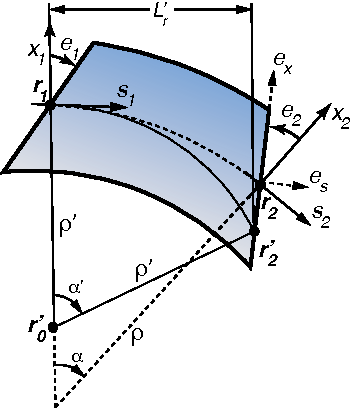
\includegraphics{bend-vary1.pdf}
    \caption{
With \vn{fiducial_pt} set to \vn{entrance_end}, $\bfr_1$ is the fiducial point at the entrance
end.  By construction, the entrance point $\bfr_1$ and the
slope of the reference curve at $\bfr_1$ is invariant with the reference curve before (dashed line)
and after (solid line) being tangent to $\bfs_1$ where $\bfs_1$ being the perpendicular to $\bfx_1$.
    }
    \label{f:bend.fid1}
  \end{subfigure}
  \hfill
  \begin{subfigure}[b]{0.4\textwidth}
    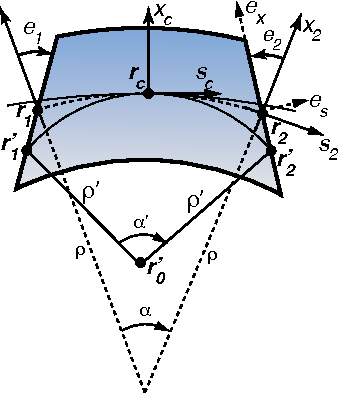
\includegraphics{bend-vary2.pdf}
    \caption{
With \vn{fiducial_pt} set to \vn{center}, $\bfr_c$ is the fiducial point at the center. By
construction, the reference curve always goes through $\bfr_c$ and the tangent of the reference
curve at $\bfr_c$ is invariant.}
    \label{f:bend.fid2}
  \end{subfigure}
  \hfill
  \caption{
Geometry with \vn{fiducial_pt} set to (a) \vn{entrance_end} and (b) \vn{center}. In both cases,
$\bfr_1$ and $\bfr_2$ are the entrance and exit reference points before and $\bfr'_1$ and $\bfr_2$
are the entrance and exit points after variation of one of \vn{rho}, \vn{g}, \vn{b_field}, or
\vn{angle}.  Similarly, $\rho$ and $\alpha$ are the bending radius and bending angle before
variation while $\rho'$ and $\alpha'$ are the bending radius afterwards.  Finally, $e_1$ $e_2$
are the face angles and rectangular length before variation, and $L'_r$ and $\bfr'_0$ are the
rectangular length and center of curvature after variation.
  }
  \label{f:bend.fid}
\end{figure}

\fig{f:bend.fid} shows the situation when the \vn{fiducial_pt} is set to either \vn{entrance_end} or
\vn{center} (the situation for the \vn{exit_end} setting is analogous to the \vn{entrance_end}
setting and so is not discussed). For any one of the \vn{fiducial_pt} settings discussed there are
essentially two cases. One case is direct variation of the bend field via variation of \vn{rho},
\vn{g}, or \vn{b_field}. This is called ``\vn{g}-variation''. The other type of variation is
variation of \vn{angle}. This is called ``angle-variation''. The discussion below shows how, with
\vn{g}-variation, \vn{l}, \vn{e1}, and \vn{e2} are calculated. With \vn{angle}-variation, \vn{l},
\vn{g}, \vn{e1}, and \vn{e2} need to be calculated. Once \vn{l} and \vn{g} are know, the other
parameters \vn{l_chord}, \vn{l_rectangle}, \vn{l_sagitta} (and \vn{angle} for the \vn{g}-variation
case) can be readily computed.

The \vn{entrance_end} analysis is as follows (\fig{f:bend.fid1}). The entrance end coordinates
around the point $\bfr_1$ are held fixed and as as a result $\bfr'_1 = \bfr_1$ and \vn{e1} does not
vary as well. $\bfr_2$ is the exit point before variation and $\bfr_3$ is the exit point after. The
position of $\bfr_3$ is calculated by first calculating the position of $\bfr_1$ in a coordinate
system centered at $\bfr_2$ and with axes parallel to the $(\bfs_1, \bfx_1)$ axes of the coordinate
system at $\bfr_1$
\begin{equation}
  \bar\bfr_1 = \left( -l_{\text{rectangle}}, \rho \, (1 - \cos\alpha) \right)
\end{equation}
Where the bar denotes that the coordinates are in the $(\bfs_1, \bfx_1)$ system.
The coordinates of $\bfr_1$ in the $(\bfe_s, \bfe_x)$ coordinate system
with origin at $\bfr_2$ and with $\bfe_x$ along the bend edge and $\bfe_s$ perpendicular to $\bfe_x$
is a rotation $\bfR(\theta)$ 
\begin{equation}
  \bfr_1 = \bfR(\alpha - e_2) \, \bar\bfr_1
\end{equation}
The angle $\theta_1$ of the vector $\bfs_1$, which is the invariant tangent of the reference curve
at the point $\bfr_1$, in the $(\bfe_s, \bfe_x)$ coordinate system (which is used from here on) is
\begin{equation}
  \theta_1 = \alpha - e_1
\end{equation}
The center of curvature after variation $\bfr'_0$ is 
\begin{equation}
  \bfr'_0 = \bfr_1 + \rho' \, \left( \sin\theta_1, -\cos\theta_1 \right)
\end{equation}
The reference trajectory after variation $\bfr'$ is a circular arc subject to the condition
\begin{equation}
  \left| \bfr' - \bfr'_0 \right| = \rho'^2
  \label{rr0r}
\end{equation}
With \vn{g}-variation, the value of $\rho'$ is set (perhaps indirectly) by the User. To find the
point $\bfr'_2$, it is noted that in the $(e_s, e_x)$ coordinate system,  the $s$
coordinate of $\bfr'_2$, $r'_{2s}$ is zero.
so using this in\Eq{rr0r} and throwing away the unphysical root gives for the $x$ coordinate
\begin{equation}
  r'_{2x} = r_{1x} + \frac{2 \, c}{-b - \sqrt{b^2-4 \, a \, c}}
\end{equation}
where
\begin{align}
  a &= g' \CRNO
  b &= 2 \, \cos\theta_1 \\
  c &= g' \, r_{1s}^2 + 2 \, r_{1s} \, \sin\theta_1 \nonumber
\end{align}
where $g' = 1 / \rho'$.
The rectangular length after variation $L'_r$ is then
\begin{equation}
  L'_r = L_r + r'_{2x} * \sin\theta_1
\end{equation}
where $L_r$ is the rectangular length before variation.
Finally, the length $L'$ after variation is
\begin{equation}
  L' = \text{asinc} \left( g' \, L'_r \right) \, L'_r
\end{equation}
where $\text{asinc}$ is the function
\begin{equation}
  \text{asinc}(\theta) = \frac{\sin^{-1}(\theta)}{\theta}
\end{equation}

For \vn{fiducial_pt} set to \vn{entrance_end} and with \vn{angle}-variation, $\alpha'$ is know and
$g'$ can be computed via
\begin{equation}
  g' = \frac{\sin(\alpha' - \theta_1) + \sin(\theta_1)}{r_{1s}}
  \label{gatt}
\end{equation}
With this, all other parameters can be created. In both \vn{angle}-variation and \vn{g}-variation the new
face angle $e'_2$ is given by
\begin{equation}
  e'_2 = e_2 + \alpha' - \alpha
\end{equation}

For \vn{fiducial_pt} set to \vn{center}, The center point $\bfr_c$ (see \fig{f:bend.fid2}) is held
constant.  Here the \vn{g}-variation analysis is similar to the \vn{g}-variation analysis with
\vn{fiducial_pt} set to \vn{entrance_end} (or \vn{exit_end} except in this case the reference orbit
to the right and left of $bfr_c$ are analyzed separately and the two lengths for each piece are
added together. For \vn{angle}-variation, the only situation where it is possible to keep $\bfr_c$
fixed while varying the angle is when \vn{e1} and \vn{e2} are equal. In this instance, the
calculation is again similar to the \vn{angle}-variation analysis with the \vn{fiducial_pt} set to
either end. If \vn{e1} and \vn{e2} are not equal, a calculation is done that gives the desired angle
but the center point will shift.

%---------------------------------------------------------------------------------
%---------------------------------------------------------------------------------
\section{Converter Tracking}
\label{s:converter.track}
\index{converter} 

Tracking through a \vn{converter} element involves generating five random numbers
  \footnote{
Since the outgoing particle starts at the exit surface of the converter only five numbers
are needed to generate the 6-dimensional particle phase space position.
  }
and then using these numbers with the outgoing particle distribution to generate the position and
orientation of the outgoing particle. The outgoing particle distribution is pre-computed by a
program \vn{converter_element_modeling} and the distribution parameters are included in the
converter element description in the \bmad lattice file (\sref{s:converter}). The accuracy of the
converter modeling will depend in part upon the granularity of the probability tables generated
by the \vn{converter_element_modeling} program and on other approximations made during
tracking. Generally, inaccuracies in the 1\% to 10\% range are to be expected.

In a tracking simulation, a single outgoing particle is generated for each incoming particle. Since,
in a real machine, the number of outgoing particles will not be equal to the number of incoming
particles, each outgoing particle is assigned a weight such that the weighted distribution of
outgoing particles is correct. This weight will be the same for all outgoing particles. The weight
will depend upon whether the momentum or angular range of the outgoing particles is restricted using
the element parameters (\sref{s:converter}):
\begin{example}
  pc_out_min    ! Minimum momentum of generated outgoing particles (eV).
  pc_out_max    ! Maximum momentum of generated outgoing particles (eV).
  angle_out_max ! Maximum angle to the surface perpendicular (rad).
\end{example}

%-------------------------------------------------------------------------

\begin{figure}[tb]
  \centering
  \includegraphics[width=5in]{converter.pdf}
  \caption[Converter geometry.]
  {
An incoming particle strikes the bottom of the converter. At some point within the interior, a new
particle is generated and this new particle exits the top surface. To calculate the position and
orientation of the outgoing particle, a coordinate system is established where the origin point
$\wt\calO$ is the point that the incoming particle would strike the top surface if it went straight
through and the $(x,y)$ axes are randomly rotated with respect to the $(x_b,y_b)$ body coordinate axes.
By construction, the position of the outgoing particle will be along the $x$-axis.
  }
  \label{f:converter}.
\end{figure}

%-------------------------------------------------------------------------

The geometry of the converter is shown in \fig{f:converter}. On the top surface, where the outgoing
particle emerges, $(x_b,y_b)$ are the axes for the element body coordinate system (\sref{s:coords.3}).
To generate the position and orientation of the outgoing particle, another coordinate system is used
with axes labeled by $(x,y)$. Each outgoing particle will be assigned its own $(x,y)$
axes. The origin $\wt\calO$ of this coordinate system is constructed by placing $\wt\calO$ at the
point where the incoming particle under consideration would strike the top surface if the incoming
particle would pass straight through the converter. The angular orientation of the $(x,y)$ axes
with respect to the $(x,y)$ axes is chosen using a random number with a uniform probability
distribution in the interval $[0, \pi]$. By construction, the outgoing particle, at the surface of
the converter will be generated at a point a distance $r$ along the $x$-axis.

The particle distribution is calculated at a number of converter thickness $t_i$, $i = 1 \ldots
N_t$. It is an error if the actual converter thickness is outside the range of these
thicknesses. [The exception is if only one distribution for a given thickness is present, this
distribution is used to generate the outgoing particle coordinates independent of the converter
thickness.]  The particle distribution is also calculated within a certain incoming particle
momentum range. It is also an error if an incoming particle has a momentum outside of this range.

The first step is to choose the value of the outgoing particle's momentum $p_\txt{out}$. For each
thickness $t_i$, the pre-computed particle distribution parameters includes a two-dimensional table
of $P(p_\txt{out}, r)$ --- the probability density of creating an outgoing particle versus
$p_\txt{out}$ and $r$. $P(p_\txt{out},r)$ is normalized so that the integrated probability is equal
to the average number of outgoing particles created for each incoming particle $N_\txt{out}/N_{in}$
\begin{equation}
  \frac{N_\txt{out}}{N_{in}} = \int \int dp_\txt{out} \, dr \, P(p_\txt{out}, r)
  \label{nnprp}
\end{equation}
The integrals are done using linear interpolation between grid points.  From a $P(p_\txt{out},r)$
probability table, a ``normalized'' probability $P_\txt{n}(p_\txt{out},r)$ table is computed where
$P_\txt{n}$ is the probability of generating a particle at given $p_\txt{out}$ and $r$ with an
angular range restricted by \vn{angle_out_max}. If \vn{angle_out_max} is not set, $P_\txt{n}$ will
be equal to $P$.  This calculation is part of a ``setup'' computation done before tracking which, to
save time, is only done if one of the three element parameters, \vn{pc_out_min}, \vn{pc_out_max}, or
\vn{angle_out_max}, changes. Additionally, the setup includes creating a table of $I(p_\txt{out})$
which is the integrated probability for generating a particle with momentum less than $p_\txt{out}$
\begin{equation}
  I_p(p_\txt{out}) = \frac{\dstyle \int_{p_\txt{min}}^{p_\txt{out}} d\pw_\txt{out} 
  \int dr \, P_\txt{n}(\pw_\txt{out}, r)}
  {\dstyle \int_{p_\txt{min}}^{p_\txt{max}} d\pw_\txt{out} \int dr \, P_{n}(\pw_\txt{out}, r)}
\end{equation}
where $p_\txt{min}$ is the minimum momentum in the $P(p_\txt{out}, r)$ table or the value of
\vn{pc_out_min} which ever is greatest and $p_\txt{max}$ is the maximum momentum in the
$P(p_\txt{out}, r)$ table or the value of \vn{pc_out_max} which ever is smallest. $I(p_\txt{out})$
is normalized such that $I(p_\txt{max}) = 1$. A value for $p_\txt{out}$ is generated by solving
numerically for $p_\txt{out}$ the equation
\begin{equation}
  I_p(p_\txt{out}) = R_1
\end{equation}
where $R_1$ is a random number with uniform distribution in the interval $[0,1]$.  This
calculation is done for the two $t_i$ thicknesses that straddle the actual thickness. The value of
$p_\txt{out}$ assigned to the outgoing particle is obtained via linear interpolation between the two
computed values. Note that for both thicknesses the same random number needs to be used.

The next step is to choose a value for $r$. This is done by solving the equation
\begin{equation}
  I_r(r) = R_2
\end{equation}
where $R_2$ is another random number with uniform distribution in the interval $[0,1]$ and $I_r$ is 
\begin{equation}
  I_r(r) = \frac{\dstyle \int_0^r d\rw \, P_\txt{n}(p_\txt{out}, \rw)}
  {\dstyle \int_0^{r_\txt{max}} d\rw \, P_{n}(p_\txt{out}, \rw)}
\end{equation}
with $p_\txt{out}$ being the momentum chosen for the particle and $r_\txt{max}$ being the maximum
radius the probability table goes out to\footnote
  {
The range $[0,r_\txt{max}]$ encompasses nearly all of the outgoing particles. In principle, the
integral could be extended by extrapolating the values in the table but this could potentially lead
to inaccuracies in determining the outgoing orientation. Generally the inaccuracy in truncating the
distribution at $r_\txt{max}$ should be small.
  }. 
Like $p_\txt{out}$, this calculation is done for the two
$t_i$ thicknesses that straddle the actual thickness. The value of $r$ assigned to the outgoing
particle is obtained via linear interpolation between the two computed values. Note that for both
thicknesses the same random number needs to be used.

Once $p_\txt{out}$ and $r$ have been chosen, the next steps are to choose values for the angular
orientation of the outgoing particle. The angular orientation is characterized by the distribution
parameters using the derivatives $x' = dx/ds$ and $y' = dy/ds$ in the form of a skewed Lorentzian
probability distribution $P_d$
\begin{equation}
  P_d\left( x', y' ; p_\txt{out}, r \right) =
  A_d \, \frac{1 + \beta \, x'}{1 + \alpha_x^2 \, \left( x' - c_x \right)^2 +
  \alpha_y^2 \, \left( y' \right)^2}
  \label{pxsxs}
\end{equation}
where the parameters $A_d$, $\beta$, $c_x$, $\alpha_x$, and $\alpha_y$ all depend upon $p_\txt{out}$
and $r$. Notice that by construction, with the outgoing particle generated on the $x$-axis, the
distribution is symmetric about $y'$-axis. The pre-computed distribution characterizes each of these
parameters by a set of one or more fits which are functions of $p_\txt{out}$ and $r$. There are also
four functions of $p_\txt{out}$ and $r$ that give the range over which \Eq{pxsxs} is valid
$x'_\txt{min}$, $x'_\txt{max}$, $y'_\txt{min}$, and $y'_\txt{max}$. By symmetry, $y'_\txt{min} =
-y'_\txt{max}$. Also $A_d$ can be computed from knowledge of $\beta$, $c_x$, $\alpha_x$, and
$\alpha_y$ using the normalization condition that at any given $p_\txt{out}$ and $r$
\begin{equation}
  1 = \int_{x'_\txt{min}}^{x'_\txt{max}} dx' 
  \int_{-y'_\txt{max}}^{y'_\txt{max}} dy' \, P_d \left( x', y' \right)
\end{equation}
Thus there are only seven independent parameters that need to be fitted. The fit functions for all
seven have the same form. The fit is divided into two regions. For $p_\txt{out}$ lower than some
cutoff, a parameter is fit using a set of one-dimensional functions $\Gamma_i(r)$ at discrete momentum $p_i$,
$i = 1, \ldots, N_\beta$ with
\begin{equation}
  \Gamma_i(r) = \sum_{n=1}^M c_{n,i} \, r^n
  \label{gcr}
\end{equation}
The polynomial cutoff $M$ is 4 for $c_x$ and $\beta$ and is 3 for the other five.  To evaluate a
parameter at momenta lower than $p_{N_\beta}$, the $\Gamma_i$ are used with linear interpolation in
$p$ between functions of different $p_i$. At higher energies, the parameter variation is smoother so
a two dimensional fit $Xi$ is used
\begin{equation}
  \Xi(p_\txt{out},r) = e^{-(k_p \, p_\txt{out} + k_r \, r)} \,
  \left( \sum_{n=0}^3 k_{n} \, r^n \right) \, 
  \left( 1 + \sum_{n=1}^3 w_{n} \, p_\txt{out}^n \right) + C
  \label{xkpkr}
\end{equation}
The $C$ parameter is only nonzero for $x'_\txt{min}$. 

Once $A_d$, $\beta$, $c_x$, $\alpha_x$, and $\alpha_y$ have been calculated for a given $p_\txt{out}$ and
$r$, The calculation of $x'$ starts with integrating $P_d$ in \Eq{pxsxs} over $y'$
\begin{align} 
  I_{xd} (x') &\equiv \int_{-y'_\txt{lim}}^{y'_\txt{lim}} dy' \, P_d(x', y')
  \label{ixdyp} \\
  &= 2 \, A_d \, \frac{1 + \beta \, x'}{\alpha_y \, \sqrt{1 + \alpha_x^2 \, (x' - c_x)^2 }} \,
  \tan^{-1} \left( \frac{\alpha_y \, y'_\txt{lim}}{\sqrt{1 + \alpha_x^2 \, (x' - c_x)^2}} \right)
  \nonumber
\end{align}
where $y'_\txt{lim}$ is either the lesser of $y'_\txt{max}$ and $\tan^{-1}(\text{angle_out_max})$.
A spline fit is used to integrate $I_{xd}$ and this is used to choose a value for $x'$. Once $x'$
is known, The integral of $P_d(x', y')$ over $y'$ is used to choose a value for $y'$.

Except for the placement of $\wt\calO$, the above algorithm for calculating the position and
orientation of the outgoing particle will be independent of the angular orientation of the incoming
particle. This is valid for incoming particles that are traveling perpendicular to the converter
surface. To the extent that the incoming particles are not perpendicular to the converter, this will
introduce inaccuracies. Typically, however, the incoming particles will be fairly close to being
perpendicular. Considering this, and considering the approximations used to calculate the
distribution parameters, the neglect of incoming particle orientation effects is usually justified.

%---------------------------------------------------------------------------------
%---------------------------------------------------------------------------------
\section{Drift Tracking}
\label{s:drift.std}
\index{drift} 

\bmad uses the exact map for a drift
This gives the map
\begin{align}
  x_2    &= x_1 + \frac{L \, p_{x1}}{p_l} \CRNO
  p_{x2} &= p_{x1}  \CRNO
  y_2    &= y_1 + \frac{L \, p_{y1}}{p_l} \CRNO
  p_{y2} &= p_{y1}  \\
  z_2    &= z_1 + \left( \frac{\beta}{\beta_\REF} - \frac{1 + p_{z1}}{p_l} \right) \, L \CRNO
  p_{z2} &= p_{z1} \nonumber
\end{align}
where $\beta$ is the normalized particle velocity, $\beta_\REF$ is the reference particle's
normalized velocity, and $p_l$ is the normalized longitudinal momentum 
\begin{equation}
  p_l \equiv \frac{P_l}{P_0} = \sqrt{(1 + p_z)^2 - p_x^2 - p_y^2}
\end{equation}
with $P_l$ being the longitudinal momentum.

%---------------------------------------------------------------------------------
%---------------------------------------------------------------------------------
\section{ElSeparator Tracking}
\label{s:elsep.std}
\index{elseparator}

\begin{figure}[tb]
  \centering
  \includegraphics[width=5in]{elseparator.pdf}
  \caption[ElSeparator electric field.]
  {
Elseparator Electric field. The fringe field lines break the
translational invariance in $x$.
  }
  \label{f:elsep}.
\end{figure}

[Thanks to \'Etienne Forest for the derivation of the elseparator equation of motion.]

The Hamiltonian for an electric separator is 
\begin{equation}
  H = -p_s 
  = - \left\{ \left( \frac{1}{\beta_0} + \delta + k_E \, x \right)^2 - 
  \wt m^2 - p_x^2 - p_y^2 \right\}^{1/2}
  \label{hp1b}
\end{equation}
Here the canonical coordinates $(-c \, t, \delta$ are being used, $\wt m$ is defined in \Eq{mmccp},
and $p_s = -H$ is just the longitudinal momentum.  In the above equation, $k_E$ is the normalized
field
\begin{equation}
  k_E = \frac{q \, E}{P_0 \, c}
\end{equation}
The field is taken to be pointing along the $x$-axis with positive $k_E$ accelerating a particle in
the positive $x$ direction. To solve the equations of motion, a ``hard edge'' model is used where
$k_E$ is constant inside the separator and the field ends abruptly at the separator edges.

\index{solenoid}
Since, as shown in \fig{f:elsep}, the fringe fields break the translational invariance in $x$, it is
important here that the $x = 0$ plane be centered within the separator plates. With this, the
canonical momentum $\delta$ just outside the separator assumes its free space form of $\delta = (E -
E_0) / E_0)$. This is analogous to the case of a \vn{solenoid} where, to ensure that the canonical
transverse momenta assume their free space form just outside the solenoid, the $\Bf z$-axis must be
along the centerline of the solenoid.

The solution of the equations of motion is:
\begin{align}
  x   &= (x_0 - x_c) \, \cosh \left( \frac{k_E \, L}{p_s} \right) + 
         \frac{p_{x0}}{k_E} \, \sinh \left( \frac{k_E \, L}{p_s} \right) + x_c \CRNO
  p_x &= k_E \, (x_0 - x_c) \, \sinh \left( \frac{k_E \, L}{p_s} \right) + 
         {p_{x0}} \, \cosh \left( \frac{k_E \, L}{p_s} \right) \CRNO
  y   &= y_0 + L \, \frac{p_{y0}}{p_s} \label{xxlp} \\
  p_y &= p_{y0} \CRNO
  c \, \delta t &=  \int_0^L -\frac{\partial H}{\partial \delta}
      = (x_0 - x_c) \, \sinh \left( \frac{k_E \, L}{p_s} \right) +
        \frac{p_{x0}}{k_E} \, \left[ \cosh \left( \frac{k_E \, L}{p_s} \right) - 1 \right]
        \nonumber
\end{align}
where the critical position $x_c$ is
\begin{equation} 
  x_c = -\frac{\wt E}{k_E}
\end{equation}
and 
\begin{equation}
  \wt E \equiv \frac{1}{\beta_0} + \delta = \frac{E}{P_0 \, c}
\end{equation}
 
\Eqs{xxlp} predict that for $x < x_c$ and $p_{x0} = 0$ a particle will, unphysically, accelerate in
the negative $x$ direction. In actuality, a particle in this instance will be reflected backwards by
the longitudinal component of the edge field. Specifically, the argument of the square root in
\Eq{hp1b} must be non-negative and a particle will only make it through the separator if
\begin{equation}
  x_0 > \frac{1}{k_E} \, \left( \sqrt{\wt m^2 + p_{x0}^2 + p_{y0}^2} - \wt E \right)
\end{equation}

%---------------------------------------------------------------------------------
%---------------------------------------------------------------------------------
\section{Foil Tracking}
\label{s:foil.std}
\index{foil}

A particle going through a \vn{foil} element is scattered both in angle and in energy, and the
charge of the particle may be affected. The following two subsections give the formulas used for
scattering and energy loss. Currently, the final charge is a fixed number but that may change in the
future.

%---------------------------------------------------------------------------------
\subsection{Scattering in a Foil}
\label{s:foil.scatter}

For the angle scattering, the user can select between one of two algorithms, both
of which are given in the paper by Peralta and Louro\cite{b:peralta} (also see Lynch and Dahl\cite{b:lynch})
Both methods vary the phase space $p_x$ and $p_y$ coordinates using:
\begin{equation}
  (dp_x, dp_y) = \frac{p \, \sigma}{P_0} \, (r_1, r_2)
  \label{dpr1s}
\end{equation}
where $p$ is the
particle momentum, $P_0$ is the reference momentum, $r_1$ and $r_2$ are Gaussian random numbers with
unit sigma and zero mean, and $\sigma$ is the sigma of the angular scattering distribution. The
factor of $p/P_0$ is due to a translation between change in angle and change in phase space momenta
(see \Eq{xpa1p}). 

The \vn{Highland} algorithm uses Eq.~(32) of Peralta and Louro\cite{b:peralta} to calculate the
scattering sigma:
\begin{equation}
  \sigma = \frac{(13.6 \cdot 10^6~eV) \, z}{p \, c \, \beta} \sqrt{\frac{X}{X_0}} \, \left[
  1 + 0.038 \, \ln \left( \frac{X \, z^2}{X_0 \, \beta^2} \right) \right]
  \label{sszpb}
\end{equation}
where $X_0$ is the material radiation ``length'' in kg/m$^2$, $z$ is the particle charge, $\beta$ is the particle
relativistic beta, $c$ is the speed of light, and $X$ is the foil area density in kg/m$^2$ equal
to $\rho \, t$ where $\rho$ is the material density and $t$ is the foil thickness.

The \vn{Lynch_Dahl} algorithm uses Eq.~(33) of Peralta and Louro:
\begin{equation}
  \sigma^2 = \frac{\chi_c^2}{1 + F^2} \left[ \frac{1 + \nu}{\nu} \ln (1 + \nu) - 1 \right]
  \label{sc1f}
\end{equation}
where
\begin{align}
  \nu &= \frac{0.5 \, \Omega}{(1 - F)} \CRNO
  \Omega &= \frac{\chi_c^2}{1.167 \, \chi_\alpha^2} \CRNO
  \chi_c^2 &= \left( 1.57 \cdot 10^{10} \, \frac{eV^2 \, m^2}{kg} \right) \, 
    \frac{Z (Z+1) X}{A} \left[ \frac{z}{p \, \beta} \right]^2 
  \label{no1f} \\
  \chi_\alpha &= (2.007 \cdot 10^7 \, eV^2) \, \frac{Z^{2/3}}{(p \, c)^2} 
            \left[1 + 3.34 \,  \left( \frac{Z \, z \, \alpha}{\beta} \right)^2 \right] \nonumber
\end{align}
and the $A$ is the atomic weight, $p$ is the particle momentum, $\alpha$ is the fine structure
constant, and $F$ is a fit parameter representing the percent of the central angular distribution
that is used.  $F$ is a settable parameter with a default value of 0.98.

For compound materials, the value of $X/X_0$ in \Eq{sszpb} is computed from
\begin{equation}
  \frac{X}{X_0} = \sum_{i = 1}^N \frac{X_i}{X_{0i}}
\end{equation}
where the summation is over all constituents in the material.

Also for compound materials, $\chi_c^2$ in \Eqs{sc1f} and \eq{no1f} is replaced by the sum of the
constituent $\chi_{ci}^2$, and $\chi_\alpha$ is computed from Lynch and Dahl Eq.~(11)
\begin{equation}
  \ln ( \chi_\alpha ) = \left. \sum_{i=1}^N \frac{Z_i (Z_i + 1) X_i}{A_i} \ln(\chi_{\alpha i}) \middle/
  \sum_{i=1}^N \frac{Z_i (Z_i + 1) X_i}{A_i} \right.
\end{equation}

The actual scattering distribution has $1/\theta^4$ tails ($\theta$ is the scattering angle) due to
single event large angle scattering (Rutherford scattering). By assuming a Gaussian distribution,
these tails are not present in a simulation. It is also important to note that with both the
\vn{Highland} and \vn{Lynch_Dahl} algorithms, simulating the passage of particles through a single
foil versus two foils with half the thickness as the single foil will not give exactly the same
results. This is just a reflection that both algorithms are trying to model an inherently non-Gaussian
process.

%---------------------------------------------------------------------------------
\subsection{Energy Loss in a Foil}
\label{s:foil.eloss}

The particle energy loss per unit length $dE/dx$ through a foil is calculated using the \vn{Bethe-Bloch} formula
\begin{equation}
  - \left\langle\frac{dE}{dx}\right\rangle = 
  \frac{4 \pi}{m_e c^2} \cdot \frac{nz^2}{\beta^2} \cdot \left(\frac{e^2}{4\pi\varepsilon_0}\right)^2 \cdot 
  \left[\ln \left(\frac{2m_e c^2 \beta^2}{I \cdot (1-\beta^2)}\right) - \beta^2\right]
  \label{ex4pmc}
\end{equation}
where $n$ is the material electron density, $I$ is the mean excitation energy, $z$ is the particle
charge, $c$ is the speed of light, $\epsilon_0$ is the vacuum permittivity, $\beta = {v}/{c}$, is
the normalized velocity, and $e$ and $m_e$ the electron charge and rest mass respectively.

Note that to keep the direction of travel of the particle constant when energy is lost, this implies
that $p_x/(1+p_z)$ and $p_y/(1+p_z)$ are to be held constant (\Eq{xpa1p}).

%---------------------------------------------------------------------------------
%---------------------------------------------------------------------------------
\section{Kicker, Hkicker, and Vkicker Tracking}
\label{s:kicker.std}
\index{kicker}
\index{hkicker}
\index{vkicker}
\index{elseparator}

The Hamiltonian for a horizontally deflecting kicker or separator is
\begin{equation}
  H = \frac{p_x^2 + p_y^2}{2 (1 + p_z)} - k_0 \, x 
\end{equation}
This gives the map
\begin{alignat}{2}
  x_2 &= x_1 + \frac{1}{1 + p_{z1}} \, \left( L \, p_{x1} + \frac{1}{2} k_0 \, L^2 \right), &
    p_{x2} &= p_{x1} + k_0 \, L, \CRNO
  y_2 &= y_1 + \frac{L \, p_{y1}}{1 + p_{z1}}, &
    p_{y2} &= p_{y1},  \\
  z_2 &= z_1 - \frac{L}{2 (1 + p_{z1})^2} \, 
    \left( p_{x1}^2 + p_{y1}^2 + p_{x1} \, k_0 \, L + \frac{1}{3} k_0^2 \, L^2 \right), \quad &
  p_{z2} &= p_{z1} \nonumber
\end{alignat}
The generalization when the kick is not in the horizontal plane is easily derived.

%---------------------------------------------------------------------------------
%---------------------------------------------------------------------------------
\section{LCavity Tracking}
\label{s:lcavity.std}
\index{lcavity}

%---------------------------------------------------------------------------------
\subsection{Integrating through RF fields}

When track by integrating through RF fields with \vn{field_calc} set to \vn{bmad_standard} and
\vn{tracking_method} set to something like \vn{runge_kutta}, the fields are modeled by the equations
given in Sections~\sref{s:rf.fields} and \sref{s:rf.fringe}. The \vn{bmad_standard} fields, with a
phase velocity equal to the speed of light, are appropriate for high energy particles traveling near
the speed of light. However, for lower energy particles, the actual fields in a cavity are likely to
have been designed with a lower phase velocity and this will cause a mismatch between simulation and
reality.

%---------------------------------------------------------------------------------
\subsection{kick-drift-kick model}

With \vn{bmad_standard} tracking, a kick-drift-kick model is used where the particle trajectory is modeled
such that the reference particle has a constant RF phase at the kick points even at low
velocities.\footnote
  {
Developing a 6D symplectic model which continuous acceleration and constant RF phase for the
reference particle proved too messy mainly due to the fact that at low energies it was found to
be cumbersome to calculate the appropriate RF phase at any given s-position.
  }
The cavity is divided up into equal width sections with the number of sections $N_s$ equal to the
setting of the \vn{n_rf_steps} parameter. Within a section particles are tracked as if in a field
free region (or with a solenoid component if the element's solenoid strength is non-zero). Energy
kicks are applied at the ends of the element and in between sections with the kicks at the ends
being half that of the kicks applied in the interior. The voltage (integrated field) at a kick point
is:
\begin{equation}
  V_\txt{k} = \frac{r_q \, \kappa \, V_{tot}}{N_s} \, \cos(2 \pi \, (\phi_t + \phi_\REF))
  \label{vkrq}
\end{equation}
See \Eq{dergl} for a description of the parameters in the equation. Here $\kappa$ is 0.5 for the end
kick points and is unity for interior kick points.

The reference energy in each section is adjusted to match the energy of the reference particle
(which has $\phi_t = 0$ by definition).  The reference RF phase $\phi_\REF(n)$ at a $n$\Th kick
point is obtained from the reference RF phase $\phi_\REF(0)$ at the beginning of the element with a
phase offset due to the transit time from the beginning to the kick point of the reference particle:
\begin{equation}
  \phi_\REF(n) = \phi_\REF(0) + f_\text{rf} \, \sum_{j = 1}^n t_{0j}
\end{equation}
where $t_{0j} = L / c \beta_{0j} \, N_s$ is the transit time of the reference particle across the
$j$\Th section with $L$ being the element length, and $\beta_{0j}$ the velocity of the reference
particle in the $j$\Th section. With this construction, a particle on the zero orbit will see a
constant RF phase.

Other than affecting the reference time at each kick point, the adjusting of the reference energy
in each section will affect the plotting of phase space momentum coordinates since these
are normalized to $P_0$ (\sref{s:phase.space}).

For spin tracking through the energy kick, the BMT equation is used with the integrated electric field
given by \Eq{vkrq} modeled as a field in the $z$-direction.

%---------------------------------------------------------------------------------
\subsection{Edge kick}

Cavities have a first order transverse kick in the fringe field regions at both the entrance and
exit ends due to an electric radial field 

Following the model of Rosenzweig and Serafini\cite{b:rosenzweig} (See their Eq.~(12)),
to make the fringe kick symplectic, the following Hamiltonian is used
\begin{equation}
  H_f = \mp \frac{q}{2 \, P_0 \, c} G_t \, \cos(\phi_t + \phi_\REF) \, (x^2 + y^2)
\end{equation}
where the minus sign is for the entrance end and the plus sign is for the exit end, $q$ is the
particle charge, $P_0$ is the reference momentum. Since $\phi_t = 2 \pi f_\txt{rf} \, t$ is time
dependent, it is easiest to use this Hamiltonian in energy-time phase space coordinates
(\sref{energy.phase.space}) to give the fringe kicks:
\begin{align}
  \Delta p_x &= \frac{\partial H_f}{\partial x} 
              = \mp \frac{q}{P_0 \, c} G_t \, \cos(\phi_t + \phi_\REF) \, x \CRNO
  \Delta p_y &= \frac{\partial H_f}{\partial y} 
              = \mp\frac{q}{P_0 \, c} G_t \, \cos(\phi_t + \phi_\REF) \, y \\
  \Delta p_E &= \frac{\partial H_f}{\partial \tau} 
                 = \mp \frac{\pi \, f_\txt{rf} \, q}{P_0 \, c^2} G_t \, \sin(\phi_t + \phi_\REF) \, (x^2 + y^2)
      \nonumber
\end{align}
The time shift can be thought of as due to the fact that the actual particle trajectory (and not the
averaged trajectory) has a transverse sinusodial component synced to the phase of the backwards
traveling wave.  The sinusodial component is needed to produce the pondermotive force but this
oscillation also delays the particle in time compared to the case where there is no oscillation
component.

For spin tracking through the edge field, the BMT equation is used with the integrated edge field
(voltage) $\overline{\bfE}_f$ parallel to the radius vector:
\begin{equation}
  \overline{\bfE}_f = -G_t \, \cos(\phi_t + \phi_\REF) \, (x, y, 0)
\end{equation}

%---------------------------------------------------------------------------------
\subsection{Standing wave focusing: the pondermotive force}

A \vn{LCavity}'s \vn{cavity_type} can be set to either \vn{traveling_wave} or
\vn{standing_wave}. The traveling wave cavity is modeled as single forward propagating wave while
with a the standing wave cavity, \bmad models the cavity as the superposition of a single forward
propagating wave and a single backward propagating wave. In both cases there are no harmonics.  In
both cases, it is the forward traveling wave that gives both acceleration and the edge kick.  The
difference between the two cavity types is that with a standing wave cavity, there is an extra
transverse focusing force called the ``pondermotive force''.

The time averaged transverse radial kick is modeled using R\&S Eq~(4)\footnote
  {
Notice that R\&S Eq~(4) is missing a minus sign.
  }
where, since there are no harmonics, $\eta(\phi)$ is unity (see discussion after R\&S Eq.~(13)).  In
the \bmad kick-drift-kick model, the pondermotive force is included by adding a transverse kick at
the kick points. To keep the pondermotive kick symplectic, A Hamiltonian $H_p$ is used:
\begin{equation}
  H_p = -\frac{\kappa \, L \, q^2 \, G_t^2}{16 \, N_s \, P_0^2 \, c^2 \, (1 + p_z)} \, (x^2 + y^2)
\end{equation}
Which gives kicks (using standard \bmad phase space coordinates):
\begin{align}
  \Delta p_x &= \frac{\partial H_p}{\partial x} 
              = -\frac{\kappa \, L \, q^2 \, G_t^2}{8 \, N_s \, P_0^2 \, c^2 \, (1 + p_z)} \, x \CRNO
  \Delta p_y &= \frac{\partial H_p}{\partial y} 
              = -\frac{\kappa \, L \, q^2 \, G_t^2}{8 \, N_s \, P_0^2 \, c^2 \, (1 + p_z)} \, y \\
  \Delta z &= -\frac{\partial H_p}{\partial p_z} 
              = -\frac{\kappa \, L \, q^2 \, G_t^2}{16 \, N_s \, P_0^2 \, c^2 \, (1 + p_z)^2} \, (x^2 + y^2) \nonumber
\end{align}
The kick is always focusing and is independent of any RF phase. The reason for the phase
independence is due to the fact that the phase of the backwards propagating wave with respect to the
forward propagating particle is rapidly varying. The formulas above are for the kick averaged over
all phases and therefore the phase dependence has been eliminated. Also note that the kick is
quadratic in its dependence upon $G_t$. This is similar to the transverse focusing in FODO cells
where the averaged kick is focusing and depends quadratically on the quadrupole field strength.

For spin tracking, to zeroth order, the averaged field is zero for the backwards wave so no spin
kick is applied for the backwards wave.

%-----------------------------------------------------------------------------------------
%-----------------------------------------------------------------------------------------
\section{Magnus Spin Tracking}
\label{s:magnus}

The \vn{Magnus} spin tracking method uses an analytical Magnus expansion of the T-BMT equation to
track spins.  Currently, the supported lattice elements are bends (including bends with $k_1 \neq
0$), quadrupoles, solenoids, and sextupoles.  Many other elements are treated as drifts
\sref{s:spin.methods}.

One way to obtain approximate spin-transfer maps is to truncate the flow of the T-BMT equation to a
given order in the entrance phase-space coordinates.  The SPRINT method \sref{s:sprint.std} uses
this idea at first order. The resulting map will generally not be a rotation, e.g., if quaternions
are used, the map will not have unit norm. The idea behind the Magnus expansion is to find an
approximate map which is also a rotation. Since the exact solution must be an element of the Lie
group SU(2), it can be written as $\exp(F)$, where $F$ belongs to the Lie algebra of SU(2). The
Magnus expansion provides a power expansion of $F$ which belongs to the Lie algebra of SU(2) at
every order~\cite{b:magnus}.

In SU(2), the T-BMT equation is given by Eq.~\eqref{tbmt-spinor}. This can be written in the
standard form $\Psi'(s)=A(s)\Psi(s)$. The Magnus expansion gives the second-order solution as
$\Psi(L)=\exp(F_1+F_2)\Psi(0)$, where
\begin{equation}
F_1 = \int_0^LA(s)\,ds \quad \mathrm{and} \quad F_2=\frac{1}{2}\int_0^Lds_1\int_0^{s_1}ds_2\,[A(s_1),A(s_2)].
\end{equation}
Once the trajectory through a magnet is known, $A(s)$ is known as well. We then expand $A(s)$ as a
power series in the entrance coordinates which change through the magnet (i.e, all orders of $p_z$
are retained in magnetic elements and all orders of $p_y$ are retained in a pure bend). The
truncation to first- and second-order will be written as $A^{(1)}(s)$ and $A^{(2)}(s)$,
respectively. The truncation of the exponent $F$ to second-order is then
\begin{equation}
F^{(2)}=\int_0^LA^{(2)}(s)\,ds+\frac{1}{2}\int_0^Lds_1\int_0^{s_1}ds_2\,[A^{(1)}(s_1),A^{(1)}(s_2)].
\end{equation}
The spin-transfer map is found by exponentiating $F^{(2)}$, which yields an element of SU(2) by
nature of the Magnus expansion.


%---------------------------------------------------------------------------------
%---------------------------------------------------------------------------------
\section{Octupole Tracking}
\label{s:octupole.std}
\index{octupole}

The Hamiltonian for an upright octupole is
\begin{equation}
  H = \frac{p_x^2 + p_y^2}{2 (1 + p_z)} + \frac{k_3}{24} (x^4 - 6 \, x^2 \, y^2 + y^4)
\end{equation}

An octupole is modeled using a kick-drift-kick model.

%---------------------------------------------------------------------------------
%---------------------------------------------------------------------------------
\section{Patch Tracking}
\label{s:patch.std}
\index{patch}

\begin{figure}[tb]
  \centering
  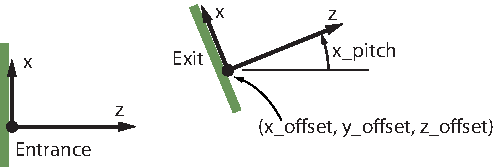
\includegraphics[width=5in]{patch.pdf}
  \caption[Standard patch transformation.]
{Standard tracking through a patch element. A particle's starting coordinate at the entrance end of
the patch has, by construction, coordinate $z$ = 0. The particle is drifted, as in a field free
region, between the entrance $z = 0$ plane and the exit $z = 0$ plane.}
  \label{f:patch.track}
\end{figure}

%---------------------------------------------------------------------------------

The transformation of the reference coordinates through a ``standard'' patch (a patch where custom
fields are not used) is given by \Eqs{vwlv} and \eq{wws}. At the entrance end of the patch, a
particle's position and momentum in the entrance coordinate system will be
\begin{alignat}{1}
  \bfr &= (x, y, 0) \CRNO
  \bfP &= (P_x, P_y, P_z) = 
    \left( p_x, p_y, \pm \sqrt{(1+p_z)^2 - p_x^2 - p_y^2} \right) \, P_{0\text{ent}}
\end{alignat}
where $p_x$, $p_y$ and $p_z$ are the phase space momenta, and $z$, which is coordinate $z$ and not
phase space $z$, is always zero by construction as shown in \fig{f:patch.track} [Also see
\fig{f:local.coords} and the discussion in \sref{s:phase.space}.] The sign of the longitudinal
momentum $P_z$ is determined by whether the particle is traveling in the positive $s$ or negative
$s$ direction (which will occur when an element is flipped longitudinally).

The transformation between entrance and exit coordinate systems is given by \Eqs{rwlr} and \eq{pps}
\begin{alignat}{1}
  \bfr &\rightarrow 
    \bfS^{-1} \, (\bfr - \bfL_\text{off}) \CRNO
  \bfP &\rightarrow \bfS^{-1} \, \bfP
\end{alignat}
where $\bfL_\text{off}$ is given by \Eq{swww}

After this transformation, the particle must be propagated by a longitudinal length
$-r_z$ to intersect the $r_z = 0$ plane of the exit face.
\begin{alignat}{1}
  \bfr &\rightarrow (r_x - r_z \, \frac{P_x}{P_z}, r_y - r_z \, \frac{P_y}{P_z}, 0) \CRNO
  \bfP &\rightarrow \bfP
\end{alignat}

The final $\bfr$ and $\bfP$ can now be used compute the particles
phase space coordinates, along with the time $t$ and the reference time
$t_\REF$ at the exit end.
\begin{alignat}{3}
  x &\rightarrow r_x \qquad &p_x &\rightarrow \frac{P_x}{P_{0\text{exi}}} \CRNO
  y &\rightarrow r_y \qquad &p_y &\rightarrow \frac{P_y}{P_{0\text{exi}}} \\
  z &\rightarrow z + r_z \, \frac{|\bfP|}{P_z} + L_0 \, \frac{\beta}{\beta_0} +
    \beta \, \text{t_offset} \qquad
    &p_z &\rightarrow \frac{(1+p_z) \, P_{0\text{ent}} - P_{0\text{exi}}}{P_{0\text{exi}}} \CRNO
  t &\rightarrow t - r_z \, \frac{|\bfP|}{P_z \, \beta} \qquad
  &t_\REF &\rightarrow t_\REF + \text{t_offset} + L_0 \, \frac{1}{\beta_0} \nonumber
\end{alignat}
where the exit reference momentum $P_{0\text{exi}}$ is related to the
entrance reference momentum $P_{0\text{ent}}$ through
\vn{e_tot_offset}.  In the above equation, $\beta$ is the particle
velocity, $\beta_0$ is the velocity of the reference particle, and
$L_0$ is the drift length of the reference particle
\begin{equation}
  L_0 = \frac{1}{S^{-1}_{33}} \, \left( 
  S^{-1}_{31} \, \text{x_offset} + S^{-1}_{32} \, \text{y_offset} + S^{-1}_{33} \, \text{z_offset}
  \right)
\end{equation}

%---------------------------------------------------------------------------------
%---------------------------------------------------------------------------------
\section{Quadrupole Tracking}
\label{s:quadrupole.std}
\index{quadrupole}

The \vn{bmad_standard} calculates the transfer map through an upright
quadrupole and then transforms that map to the laboratory frame.

The Hamiltonian for an upright quadrupole is
\begin{equation}
  H = \frac{p_x^2 + p_y^2}{2 (1 + p_z)} + \frac{k_1}{2} (x^2 - y^2)
\end{equation}
This is simply solved
\begin{align}
  x_2    &= c_x \, x_1 + s_x \, \frac{p_{x1}}{1 + p_{z1}} \CRNO
  p_{x2} &= \tau_x \, \om^2 \, \, (1 + p_{z1}) \, s_x \, x_1 + c_x \, p_{x1} \CRNO
  y_2    &= c_y \, y_1 + s_y \, \frac{p_{y1}}{1 + p_{z1}} \CRNO
  p_{y2} &= \tau_y \, \om^2 \, \, (1 + p_{z1}) \, s_y \, y_1 + c_y \, p_{y1} \\
  z_2    &= z_1 + m_{511} \, x_1^2 + m_{512} \, x_1 \, p_{x1} + m_{522} \, p_{x1}^2 + 
                   m_{533} \, y_1^2 + m_{534} \, y_1 \, p_{y1} + m_{544} \, p_{y1}^2 \CRNO
  p_{z2} &= p_{z1} \nonumber
\end{align}
where 
\begin{equation}
  \om \equiv \sqrt{\frac{|k_1|}{1 + p_{z1}}}
\end{equation}
and
\begin{alignat}{6}
         &\hspace*{3ex}  && k_1 > 0          &\hspace*{3ex}& k_1 < 0 & \qqquad
         &\hspace*{3ex}  && k_1 > 0          &\hspace*{3ex}& k_1 < 0 \CRNO
     c_x &=   && \cos  (\om \, L) && \cosh (\om \, L) & \qqquad
     c_y &=   && \cosh (\om \, L) && \cos  (\om \, L) \CRNO
     s_x &=   && \frac{\sin  (\om \, L)}{\om} && \frac{\sinh (\om \, L)}{\om} & \qqquad
     s_y &=   && \frac{\sinh (\om \, L)}{\om} && \frac{\sin  (\om \, L)}{\om} \\
  \tau_x &=   && {-}1             && {+}1             & \qqquad
  \tau_y &=   && {+}1             && {-}1             \nonumber
\end{alignat}
with this
\begin{alignat}{2}
  m_{511} &= \frac{\tau_x \,\, \om^2}{4} \, (L - c_x \, s_x) & \qqquad
  m_{533} &= \frac{\tau_y \,\, \om^2}{4} \, (L - c_y \, s_y) \CRNO
  m_{512} &= \frac{-\tau_x \,\, \om^2}{2 \, (1 + p_{z1})} \, s_x^2 & \qqquad
  m_{534} &= \frac{-\tau_y \,\, \om^2}{2 \, (1 + p_{z1})} \, s_y^2 \\
  m_{522} &= \frac{-1}{4 \, (1 + p_{z1})^2} \, (L + c_x \, s_x) & \qqquad
  m_{544} &= \frac{-1}{4 \, (1 + p_{z1})^2} \, (L + c_y \, s_y) \nonumber
\end{alignat}

%---------------------------------------------------------------------------------
%---------------------------------------------------------------------------------
\section{RFcavity Tracking}
\label{s:rfcavity.std}
\index{rfcavity}

For tracking using something like \vn{runge_kutta}, with \vn{field_calc} set to \vn{bmad_standard},
the fields are modeled by the equations given in Sections~\sref{s:rf.fields} and \sref{s:rf.fringe}.

With \vn{bmad_standard} tracking, a kick-drift-kick model is used. The kick is a
pure energy kick (see equations in \sref{s:rfcav}) and the phase of the RF is calculated under the
assumption that the waveform moves at a phase velocity equal to the velocity of the reference
particle.

With \vn{bmad_standard} tracking, the transverse forces due to the RF are ignored. This is generally
a reasonable approximation when the acceleration is small as is standard in rings. \vn{Lcavity}
elements should be used in place of \vn{rfcavity} elements when this is not so.

%---------------------------------------------------------------------------------
%---------------------------------------------------------------------------------
\section{Sad\_Mult Tracking}
\label{s:sad.mult.std}
\index{sad_mult}

The ``hard edge'' fringe field kick is taken from Forest\cite{b:forest} Eqs.~(13.29) and onward.
In the notation of \bmad, and taking into account both normal and skew terms, Eq.~(13.29)
is for the $m$\th order multipole (what Forest labels $n+1$)
\begin{equation}
  f_\pm = \mp \Re \frac{(b_m + i \, a_m) \, (x + i \, y)^{(m+1)}}{4 \, (m+2) \, (1 + p_z)}
    \left[ x \, p_x + y \, p_y + i\frac{m+3}{m+1}(x \, p_y - y \, p_x) \right]
\end{equation}

The ``soft edge'' dipole fringe for \vn{sad_mult} elements is a generalization of the soft edge
dipole fringe for a SAD bend element. For the entrance kick the equations are:
\begin{align}
  x_2 &= x_1 + \frac{\delta_1}{1 + \delta_1} \, \Delta x_{fx}, \qquad
  p_{x2} = p_{x1} + \frac{1}{1 + \delta_1} \, \left[ 
    \Delta x_{fy} \, v - \Delta x_{fay} \, v^3 \right] \CRNO
  y_2 &= y_1 - \frac{\delta_1}{1 + \delta_1} \, \Delta y_{fy}, \qquad
  p_{y2} = p_{y1} + \frac{1}{1 + \delta_1} \, \left[ 
    \Delta y_{fx} \, w - \Delta y_{fax} \, w^3 \right] \\
  z_2 &= z_1 + \frac{1}{(1 + \delta_1)^2} \, \left[ \, 
    \Delta x_{fx} \, p_{x1} - \Delta y_{fy} \, p_{y1} + 
    \frac{1}{2} \, (\Delta y_{fx} + \Delta x_{fy}) \, w^2 -
    \frac{1}{4} (\Delta y_{fax} + \Delta x_{fay}) \, w^4
    \right] \nonumber
\end{align}
where
\begin{alignat}{3}
  \Delta x_{fx}  &= \frac{K_0 \, F_B^2}{24 \, L}, & \qquad 
  \Delta y_{fx}  &= \frac{K_0^2 \, F_B}{6 \, L^2}, & \qquad 
  \Delta y_{fax} &= \frac{2 \, K_0^2}{3 \, F_B \, L^2}, \CRNO 
  \Delta y_{fy}  &= \frac{SK_0 \, F_B^2}{24 \, L}, & \qquad
  \Delta x_{fy}  &= \frac{SK_0^2 \, F_B}{6 \, L^2}, & \qquad
  \Delta x_{fay} &= \frac{2 \, SK_0^2}{3 \, F_B \, L^2}, \\
  v &= \cos\theta \, x_1 + \sin\theta \, y_1, & \qquad
  w &= -\sin\theta \, x_1 + \cos\theta \, y_1, & \qquad
  \tan\theta &= \frac{-SK_0}{K_0} \nonumber
\end{alignat}


%---------------------------------------------------------------------------------
%---------------------------------------------------------------------------------
\section{Sextupole Tracking}
\label{s:sextupole.std}
\index{sextupole}

The Hamiltonian for an upright sextupole is
\begin{equation}
  H = \frac{p_x^2 + p_y^2}{2 (1 + p_z)} + \frac{k_2}{6} (x^3 - 3 \, x \, y^2)
\end{equation}

Tracking through a sextupole uses a kick-drift-kick model.

%---------------------------------------------------------------------------------
%---------------------------------------------------------------------------------
\section{Sol\_Quad Tracking}
\label{s:sol.quad.std}
\index{sol_quad}

The Hamiltonian is
\begin{equation}
  H = \frac{(p_x + \frac{k_s }{2}\, y)^2}{2 (1 + p_z)} + 
  \frac{(p_y - \frac{k_s}{2} \, x)^2}{2 (1 + p_z)} + \frac{k_1}{2} (x^2 - y^2)
\end{equation}
Solving the equations of motion gives
\begin{align}
  x_2    &= m_{11} \, x_1 + m_{12} \, p_{x1} + m_{13} \, y_1 + m_{14} \, p_{y1} \CRNO
  p_{x2} &= m_{21} \, x_1 + m_{22} \, p_{x1} + m_{23} \, y_1 + m_{24} \, p_{y1} \CRNO
  y_2    &= m_{31} \, x_1 + m_{32} \, p_{x1} + m_{33} \, y_1 + m_{34} \, p_{y1} \CRNO
  p_{y2} &= m_{41} \, x_1 + m_{42} \, p_{x1} + m_{43} \, y_1 + m_{44} \, p_{y1} \\
  z_2    &= z_1 + \sum_{j = 1}^4 \sum_{k = j}^4 m_{5jk} \, r_j \, r_k  \CRNO
  p_{z2} &= p_{z1} \nonumber
\end{align}
where
\begin{alignat}{2}
  m_{11} &= \frac{1}{2 \, f} \, \left( f_{0+} \, c + f_{0-} \, c_h \right) & \qqquad
  m_{31} &= -m_{24} \CRNO
  m_{12} &= \frac{1}{2 \, f \, (1 + p_{z1})} \, 
            \left( \frac{f_{++}}{\om_+} \,  s + \frac{f_{--}}{\om_-} \, s_h \right) & \qqquad
  m_{32} &= -m_{14} \CRNO
  m_{13} &= \frac{\ks}{4 \, f} \, 
            \left( \frac{f_{+-}}{\om_+} \, s +\frac{f_{-+}}{\om_-} \, s_h \right) & \qqquad
  m_{33} &= \frac{1}{2 \, f} \, \left( f_{0-} \, c + f_{0+} \, c_h \right) \CRNO
  m_{14} &= \frac{\ks}{f \, (1 + p_{z1})} \, \left( -c + c_h \right) & \qqquad
  m_{34} &= \frac{1}{2 \, f \, (1 + p_{z1})} \, 
            \left( \frac{f_{+-}}{\om_+} \, s + \frac{f_{-+}}{\om_-} \, s_h \right) \CRNO
  m_{21} &= \frac{-(1 + p_{z1})}{8 \, f} \, 
            \left( \frac{\xi_{1+}}{\om_+} \, s + \frac{\xi_{2+}}{\om_-} s_h \right) & \qqquad
  m_{41} &= -m_{23} \\
  m_{22} &= m_{11} & \qqquad
  m_{42} &= -m_{13} \CRNO
  m_{23} &= \frac{\ks^3 \, (1 + p_{z1})}{4 \, f} \, \left( c - c_h \right) & \qqquad
  m_{43} &= \frac{-(1 + p_{z1})}{8 \, f} \, 
            \left( \frac{\xi_{1-}}{\om_+} \, s + \frac{\xi_{2-}}{\om_-} \, s_h \right) \CRNO
  m_{24} &= \frac{\ks}{4 \, f} \, 
            \left( \frac{f_{++}}{\om_+} \, s + \frac{f_{--}}{\om_-} \, s_h \right) & \qqquad
  m_{44} &= m_{33} \nonumber
\end{alignat}
and
\begin{alignat}{2}
  \kone        &= \frac{k_1}{1 + p_{z1}} & \qqquad 
  \ks          &= \frac{k_s}{1 + p_{z1}} \CRNO
  f            &= \sqrt{\ks^4 + 4 \, \kone^2} & \qqquad
  f_{\pm0}     &= f \pm \ks^2 \CRNO
  f_{0\pm}     &= f \pm 2 \, \kone & \qqquad
  f_{\pm\pm}   &= f \pm \ks^2 \pm 2 \, \kone \CRNO
  \om_+        &= \sqrt{\frac{f_{+0}}{2}} & \qqquad
  \om_-        &= \sqrt{\frac{f_{-0}}{2}} \\
  s            &= \sin (\om_+ \, L) & \qqquad
  s_h          &= \sinh (\om_- \, L) \CRNO
  c            &= \cos (\om_+ \, L) & \qqquad
  c_h          &= \cosh (\om_- \, L) \CRNO
  \xi_{1\pm} &= \ks^2 \, f_{+\mp} \pm 4 \, \kone \, f_{+\pm} & \qqquad
  \xi_{2\pm} &= \ks^2 \, f_{-\pm} \pm 4 \, \kone \, f_{-\mp} \nonumber
\end{alignat}

The $m_{5jk}$ terms are obtained via \Eq{zz121p}
\begin{align}
  m_{5jk} = - \frac{\tau_{jk}}{2 (1 + p_{z1})^2} \int \! ds \, 
  & \left[ 
    \left( m_{2j} + \frac{k_s}{2} \, m_{3j} \right) \, 
    \left( m_{2k} + \frac{k_s}{2} \, m_{3k} \right)   
  \right. + \\
  & \hspace*{15ex} \left.
    \left( m_{4j} - \frac{k_s}{2} \, m_{1j} \right) \, 
    \left( m_{4k} - \frac{k_s}{2} \, m_{1k} \right) 
  \right] \nonumber
\end{align}
where
\begin{equation}
  \tau_{jk} = 
  \begin{cases}
    1 & j = k \\
    2 & j \ne k 
  \end{cases}
\end{equation}
The needed integrals involve the product of two trigonometric or
hyperbolic functions. These integrals are trivial to do but the
explicit equations for $m_{5jk}$ are quite long and in the interests of
brevity are not reproduced here.

%---------------------------------------------------------------------------------

\begin{figure}[tb]
  \centering
  \includegraphics[width=5in]{solenoid.pdf}
  \caption[Solenoid with a hard edge.]
  {
Solenoid with a hard edge. The field is assumed to end abruptly at the edges of the solenoid. Here,
for purposes of illustration, the field lines at the ends are displaced from one another.
  }
  \label{f:solenoid}.
\end{figure}

%---------------------------------------------------------------------------------
\section{Solenoid Tracking}
\label{s:solenoid.std}
\index{solenoid}

The \vn{bmad_standard} solenoid tracking does not make the small angle approximation.
The transfer map for the solenoid is:
\begin{align}
  x_2    &= \frac{1 + c}{2} \, x_1 + \frac{s}{k_s} \, p_{x1} +
           \frac{s}{2} \, y_1 + \frac{1 - c}{k_s} \, p_{y1} \CRNO
  p_{x2} &= \frac{-k_s \, s}{4} \, x_1 + \frac{1 + c}{2} \, p_{x1} - 
           \frac{k_s \, (1 - c)}{4} \, y_1 + \frac{s}{2} \, p_{y1} \CRNO
  y_2    &= \frac{-s}{2} \, x_1 - \frac{1 - c}{k_s} \, p_{x1} +
           \frac{1 + c}{2} \, y_1 + \frac{s}{k_s} \, p_{y1} \\      
  p_{y2} &= \frac{k_s \, (1 - c)}{4} \, x_1 + \frac{-s}{2} \, p_{x1} -
            \frac{k_s \, s}{4} \, y_1 + \frac{1 + c}{2} \, p_{y1} \CRNO 
  z_2    &= z_1 + L \left( \frac{\beta}{\beta_0} - \frac{1+p_z}{p_r} \right) \CRNO
  p_{z2} &= p_{z1} \nonumber
\end{align}
where $k_s = q \, B/P_0$ is the normalized field and
\begin{align}
  c &= \cos \left( k_s L / p_r \right) \CRNO
  s &= \sin \left( k_s L / p_r \right)
\end{align}
with
\begin{equation}
  p_r = \sqrt{(1 + p_z)^2 - (p_x + y_1 \, k_s/2)^2 - (p_y - x_1 \, k_s/2)^2}
\end{equation}

To be useful, the canonical momenta $p_x$ and $p_y$ in the above equations must be connected to the
canonical momenta used for other elements (drifts, quadrupoles, etc.) that may be placed to either
side of the solenoid. These side elements use zero $a_x$ and $a_y$ (cf. \Eq{pmc2pc}). The vector
potential used in the solenoid canonical momenta may be made zero at the edges of the solenoid if
the solenoid fringe field is assumed to end abruptly at the edges of the solenoid (as shown in
\fig{f:solenoid}), and the reference axis $\Bf z$-axis (at $x$ = $y$ = 0) is placed along the
centerline of the solenoid so that there is cylindrical symmetry around the $\Bf z$-axis.

%-----------------------------------------------------------------------------------------
\section{Sprint Spin Tracking}
\label{s:sprint.std}
\index{sprint spin tracking}

The \vn{sprint} spin tracking method is named after the \vn{SPRINT} program developed by Matthias
Vogt.  The \vn{sprint} algorithm Uses a first order spin map evaluated with respect to the zero
orbit to track through elements. This method is much faster than PTC integration, and its run-time
does not increase proportionally to element length. Currently, the supported lattice elements are
bends (including bends with $k_1 \neq 0$), quadrupoles, and solenoids \sref{s:spin.methods}.

Elements with fringe field contributions are split into three quaternions representing the entrance,
body, and exit of the element. Before propagation, the exit fringe quaternion is always equivalent
to the entrance fringe quaternion, with all field strengths multiplied by -1, and $e_1$ replaced
with $-e_2$. The exit quaternion is then propagated to the end of the element via Bmad mapping
tools. Appropriate quaternions are concatenated according to the values of \vn{spin_fringe_on} and
\vn{fringe_at}.

\begin{alignat}{8}
 & {d}    &&= g \, l              && {e}    &&= a \, g \, l\gamma   && s     &&= a \, k_s l       && {t}    &&= (1+a) k_s l         \CRNO
 & c_{d}  &&= \cos({d})    \qquad && s_{e2} &&= \sin(\frac{{e}}{2}) && c_{s} &&= \cos({s}) \qquad && c_{t}  &&= \cos({t})           \\
 & s_{d}  &&= \sin({d})           && c_{e2} &&= \cos(\frac{{e}}{2}) && s_{s} &&= \sin({s})        && s_{t2} &&= \sin(\frac{{t}}{2}) \CRNO
 & \chi   &&= 1+a\gamma           && \zeta  &&= \gamma - 1   \qquad && \psi  &&= \gamma^2 - 1     && c_{t2} &&= \cos(\frac{{t}}{2}) \nonumber
\end{alignat}

%-----------------------------------------------------------------------------------------
\subsection{SBend Body, $k_1 = 0$}

\begin{center}
\begin{tabular}{llll} \toprule
        & $q_0$    & $q_y$     & $q_z$ \\ \midrule
  $1$   & $c_{e2}$ & $-s_{e2}$ &       \\ \addlinespace[1ex]
  $x$   & $-\frac{1}{2} g \chi s_{d} s_{e2}$ & $-\frac{1}{2} g \chi \, s_{d} c_{e2}$ & \\ \addlinespace[1ex]
  $p_x$ & $\frac{1}{2} \chi \, (c_{d} - 1)  s_{e2}$ & $\frac{1}{2} \chi \, (c_{d} - 1) c_{e2}$ & \\ \addlinespace[1ex]
  $p_y$ &          &           & $\frac{1}{\gamma} \zeta \, s_{e2}$ \\ \addlinespace[1ex]
  $p_z$ & $\frac{1}{2 \gamma} \left(\gamma \, \chi \, s_{d} -a \, \psi \, {d} \right) s_{e2}$ & & \\
  \bottomrule
\end{tabular}
\end{center}

%-----------------------------------------------------------------------------------------
\subsection{Sbend Body, $k_1 \neq 0$}

\begin{equation}
\begin{aligned}
  &  k_x = k_1 + g^2 \\
  & \omega_x = \sqrt{|k_x|} \\
  & \omega_y = \sqrt{|k_1|}
\end{aligned}
\qquad\qquad\qquad
\begin{aligned}
  & \alpha = 2(a^2 g^2 \gamma^2 + k_1) \\ \nonumber
  & \beta = a g k_1 (\gamma \chi - \zeta) \\ \nonumber
  & \sigma = \omega_y (k_1 + a k_1 \gamma + a^2g^2 \zeta \gamma)\\ \nonumber
  & \xi = \omega_y (k_1 \chi + a^2 g^2 \zeta \gamma) \nonumber
\end{aligned}
\end{equation}

\begin{center}
\begin{tabular}{cccc}
  $k_x > 0$                  & $k_x < 0$              & $k_1 > 0$                   & $k_1 < 0$  \\
  $s_x = \sin{(l \omega_x)}$ & $ \sinh{(l \omega_x)}$ & $s_y = \sinh{(l \omega_y)}$ & $ \sin{(l \omega_y)}$ \\
  $c_x = \cos{(l \omega_x)}$ & $ \cosh{(l \omega_x)}$ & $c_y = \cosh{(l \omega_y)}$ & $ \cos{(l \omega_y)}$ \\
  $\tau_x = -1$              & $+1$                   & $\tau_y = +1$               & $-1$
\end{tabular}
\end{center}

\begin{center}
\begin{tabular}{lllll} \toprule
        & $q_0$    & $q_x$ & $q_y$     & $q_z$ \\ \midrule
  1     & $c_{e2}$ &       & $-s_{e2}$ &       \\ \addlinespace[1ex]
  $x$   & $\frac{-k_x \chi}{2 \omega_x} s_x s_{e2}$            &   &
    $\frac{-k_x \chi}{2 \omega_x} s_x c_{e2}$ & \\ \addlinespace[1ex]
  $p_x$ & $\frac{k_x \chi}{2\omega_x^2} \tau_x (1-c_x) s_{e2}$ &   &
    $\frac{k_x \chi}{2 \omega_x^2} \tau_x \left(1-c_x\right) c_{e2}$ & \\ \addlinespace[1ex]
  $y$   &          &
    {$\begin{aligned}
      \frac{-1}{\alpha} &\bigl[ \beta (1+ c_y) s_{e2} +{} \\[-1.5ex]
      & \hskip4.5em \tau_y \sigma s_y c_{e2} \bigr]
    \end{aligned}$} &  &
    {$\begin{aligned}
       \frac{1}{\alpha} &\bigl[ \beta (1-c_y) c_{e2} + {} \\[-1.5ex]
       & \hskip4.5em \tau_y \sigma s_y s_{e2} \bigr]
    \end{aligned}$} \\ \addlinespace[1ex]
  $p_y$ &          &
    {$\begin{aligned}
      \frac{1}{\omega_y \alpha} &\bigl[ \xi (1 - c_y) c_{e2} - {} \\[-1.5ex]
      & \hskip5em \beta s_y s_{e2} \bigr]
    \end{aligned}$} &   &
    {$\begin{aligned}
      \frac{1}{\omega_y \alpha} &\bigl[ \xi (1+c_y) s_{e2} - {} \\[-1.5ex]
      & \hskip5em \beta s_y c_{e2}\bigr]
    \end{aligned}$} \\ \addlinespace[1ex]
  $p_z$ & $\frac{g}{2}\left(\frac{\chi s_x}{\omega_x} - \frac{a l \psi}{\gamma}\right) s_{e2}$ &    &
    $\frac{g}{2}\left(\frac{\chi s_x}{\omega_x} - \frac{a l \psi}{\gamma}\right) c_{e2}$ & \\
  \bottomrule
  \end{tabular}
\end{center}

%-----------------------------------------------------------------------------------------
\subsection{Sbend Entrance Fringe}

To calculate the exit fringe, multiply all field strengths $g$ by
-1, and replace all entrance face angles $e_1$ with exit face angles $-e_2$. The negative exit face
angle is used due to Bmad convention.
\begin{center}
  \begin{tabular}{lllll} \toprule
      & $q_0$ & $q_x$                         & $q_y$                          & $q_z$ \\ \midrule
  1   & 1     &                               &                                & \\ \addlinespace[1ex]
  $x$ &       &                               & $\frac{1}{2} \chi g \tan(e_1)$ & \\ \addlinespace[1ex]
  $y$ &       & $\frac{1}{2}(1+a)g \sin(e_1)$ &                                & $-\frac{1}{2}(1+a)g \cos(e_1)$ \\
  \bottomrule
  \end{tabular}
\end{center}

%-----------------------------------------------------------------------------------------
\subsection{Quadrupole}

\begin{equation}
  \omega = \sqrt{|k_1|} \nonumber
\end{equation}

\begin{center}
\begin{tabular}{cccc}
  $k_1 > 0$ & $k_1 < 0$ & $k_1 > 0$ & $k_1 < 0$  \\
  $s_x = \frac{\sin{(l \omega)}}{\omega}$ & $ \frac{\sinh{(l \omega)}}{\omega}$ &$s_y = \frac{\sinh{(l \omega)}}{\omega}$ & $ \frac{\sin{(l \omega)}}{\omega}$ \\
  $c_x = \frac{1 - \cos{(l \omega)}}{\omega^2}$ & $ \frac{-1 + \cosh{(l \omega)}}{\omega^2}$ &$c_y = \frac{-1 + \cosh{(l \omega)}}{\omega^2}$ & $ \frac{1 - \cos{(l \omega)}}{\omega^2}$ \\
\end{tabular}
\end{center}
\everymath{}

\begin{center}
\begin{tabular}{llll} \toprule
        & $q_0$ & $q_x$ & $q_y$ \\ \midrule
  1     & 1     &       &       \\ \addlinespace[1ex]
  $x$   &       &       & $-\frac{1}{2} k_1 \chi s_x$ \\ \addlinespace[1ex]
  $p_x$ &       &       & $-\frac{1}{2} k_1 \chi c_x$ \\ \addlinespace[1ex]
  $y$   &       & $-\frac{1}{2} k_1 \chi s_y$ & \\ \addlinespace[1ex]
  $p_y$ &       & $-\frac{1}{2} k_1 \chi c_y$ & \\
\bottomrule
\end{tabular}
\end{center}

%-----------------------------------------------------------------------------------------
\subsection{Solenoid Element Body}

\begin{center}
\begin{tabular}{lllll} \toprule
  &  $q_0$ & $q_x$ & $q_y$ & $q_z$ \\ \midrule
  1 & $c_{t2}$ & & & $-s_{t2}$ \\ \addlinespace[1ex]
  $x$ & & $\frac{1}{4} k_s \zeta ((1 - c_{s}) c_{t2} - s_{s} s_{t2})$ & $\frac{1}{4} k_s \zeta ((-1 + c_{s}) s_{t2} - s_{s} c_{t2})$ & \\ \addlinespace[1ex]
  $p_x$ & & $\frac{1}{2} \zeta ((1-c_{s}) {st2} + s_{s} c_{t2})$ & $\frac{1}{2} \zeta ((1 - c_{s}) c_{t2} - s_{s} s_{t2})$ & \\ \addlinespace[1ex]
  $y$ & & $\frac{1}{4} k_s \zeta ((1 - c_{s}) s_{t2} + s_{s} c_{t2})$ & $\frac{1}{4} k_s \zeta ((1 - c_{s}) c_{t2} - s_{s} s_{t2})$ &\\ \addlinespace[1ex]
  $p_y$ & & $\frac{1}{2} \zeta ((-1 + c_{s}) c_{t2} + s_{s} s_{t2})$ & $\frac{1}{2} \zeta ((1-c_{s}) s_{t2} + s_{s} c_{t2})$ & \\ \addlinespace[1ex]
  $p_z$ & $\frac{1}{2} {t} s_{t2}$ & & & $\frac{1}{2} {t} c_{t2}$ \\
\bottomrule
\end{tabular}
\end{center}

%-----------------------------------------------------------------------------------------
\subsection{Solenoid Entrance Fringe}
To calculate the exit fringe, multiply all field strengths $k_s$ by -1.
\begin{center}
\begin{tabular}{llll} \toprule
  & $q_0$ & $q_x$ & $q_y$ \\ \midrule
  1 & 1 & & \\
  $x$ & & $\frac{1}{4} k_s \chi $ &  \\
  $y$ & & & $\frac{1}{4} k_s \chi $ \\
\bottomrule
\end{tabular}
\end{center}

%---------------------------------------------------------------------------------
\section{Symplectic Tracking with Cartesian Modes}
\label{s:wiggler.std}
\index{wiggler!tracking}

The method for symplectic integration for elements that define the magnetic field using a
Cartesian mode decomposition (\sref{s:cart.map}) is outlined in \sref{s:symp.track}.  The
vector potential is constructed to avoid singularities when one of the wave vectors $k_x$,
$k_y$, or $k_z$ is zero.

For the \vn{x} \vn{family} the vector potential is:
\begin{center}
{
\setlength{\tabcolsep}{1pt}
\begin{tabular}{lrllrllrll}
  Form \; & \multicolumn{3}{l}{hyper-y}  & \multicolumn{3}{l}{hyper-xy}  & \multicolumn{3}{l}{hyper-x} \\
  $A_x$   & 
    $A$ & $\dfrac{k_z}{k_y^2}$      & $\Se_x \, \Sh_y \, \Se_z \qquad$ &
    $A$ & $\dfrac{1}{k_y}$          & $\Sh_x \, \Sh_y \, \Se_z \qquad$ &
    $A$ & $\dfrac{k_z}{k_x \, k_y}$ & $\Sh_x \, \Se_y \, \Se_z$ \\
  $A_y$   & 0 &&& 0 &&& 0 && \\
  $A_z$   & 
    $A$ & $\dfrac{k_x}{k_y^2}$      & $\Ce_x \, \Sh_y \, \Ce_z \qquad$ &
    $A$ & $\dfrac{k_x}{k_y \, k_z}$ & $\Ch_x \, \Sh_y \, \Ce_z \qquad$ &
    $A$ & $\dfrac{1}{k_y}$          & $\Ch_x \, \Se_y \, \Ce_z$ 
\end{tabular}
}
\end{center}

For the \vn{y} \vn{family} the vector potential is:
\begin{center}
{
\setlength{\tabcolsep}{1pt}
\begin{tabular}{lrllrllrll}
  Form \; & \multicolumn{3}{l}{hyper-y}  & \multicolumn{3}{l}{hyper-xy}  & \multicolumn{3}{l}{hyper-x} \\
  $A_x$   & 0 &&& 0 &&& 0 && \\
  $A_y$   & 
    $-A$ & $\dfrac{k_z}{k_x \, k_y}$ & $\Se_x \, \Sh_y \, \Se_z \qquad$ &
    $-A$ & $\dfrac{1}{k_x}$          & $\Sh_x \, \Sh_y \, \Se_z \qquad$ &
    $-A$ & $\dfrac{k_z}{k_x^2}$      & $\Sh_x \, \Se_y \, \Se_z$ \\
  $A_z$   & 
    $-A$ & $\dfrac{1}{k_x}$          & $\Se_x \, \Ch_y \, \Ce_z \qquad$ &
    $-A$ & $\dfrac{k_y}{k_x \, k_z}$ & $\Sh_x \, \Ch_y \, \Ce_z \qquad$ &
    $-A$ & $\dfrac{k_y}{k_x^2}$      & $\Sh_x \, \Ce_y \, \Ce_z$ 
\end{tabular}
}
\end{center}

For the \vn{qu} \vn{family} the vector potential is:
\begin{center}
{
\setlength{\tabcolsep}{1pt}
\begin{tabular}{lrllrllrll}
  Form \; & \multicolumn{3}{l}{hyper-y}  & \multicolumn{3}{l}{hyper-xy}  & \multicolumn{3}{l}{hyper-x} \\
  $A_x$   & 
     $A$ & $\dfrac{1}{k_z}$          & $\Se_x \, \Ch_y \, \Se_z \qquad$ &
     $A$ & $\dfrac{k_y}{k_z^2}$      & $\Sh_x \, \Ch_y \, \Se_z \qquad$ &
     $A$ & $\dfrac{k_y}{k_x \, k_z}$ & $\Sh_x \, \Ce_y \, \Se_z$ \\
  $A_y$   & 
    $-A$ & $\dfrac{k_x}{k_y \, k_z}$ & $\Ce_x \, \Sh_y \, \Se_z \qquad$ &
    $-A$ & $\dfrac{k_x}{k_z^2}$      & $\Ch_x \, \Sh_y \, \Se_z \qquad$ &
    $-A$ & $\dfrac{1}{k_z}$          & $\Ch_x \, \Se_y \, \Se_z$ \\
  $A_z$   & 0 &&& 0 &&& 0 &&
\end{tabular}
}
\end{center}

For the \vn{sq} \vn{family} the vector potential is:
\begin{center}
{
\setlength{\tabcolsep}{1pt}
\begin{tabular}{lrllrllrll}
  Form \; & \multicolumn{3}{l}{hyper-y}  & \multicolumn{3}{l}{hyper-xy}  & \multicolumn{3}{l}{hyper-x} \\
  $A_x$   & 
     $A$ & $\dfrac{1}{k_z}$          & $\Ce_x \, \Sh_y \, \Se_z \qquad$ &
     $A$ & $\dfrac{k_y}{k_z^2}$      & $\Ch_x \, \Sh_y \, \Se_z \qquad$ &
     $A$ & $\dfrac{k_y}{k_x \, k_z}$ & $\Ch_x \, \Se_y \, \Se_z$ \\
  $A_y$   & 
     $A$ & $\dfrac{k_x}{k_y \, k_z}$ & $\Se_x \, \Ch_y \, \Se_z \qquad$ &
    $-A$ & $\dfrac{k_x}{k_z^2}$      & $\Sh_x \, \Ch_y \, \Se_z \qquad$ &
     $A$ & $\dfrac{1}{k_z}$          & $\Sh_x \, \Ce_y \, \Se_z$ \\
  $A_z$   & 0 &&& 0 &&& 0 &&
\end{tabular}
}
\end{center}

